% ---------------------------------------------------------------------
% Real IEEE Access template (ieeeaccess.cls), sourced from the public
% erwinrmendez/ieee-access-template reference repository, which bundles
% the official class and required images (images/Logo.png,
% images/notaglineLogo.png, images/bullet.png) that this class file
% hard-codes paths to. All four files were copied to the project root.
% Front-matter macros below (\history, \doi, \address, \authorrefmark,
% \tfootnote, \markboth, \corresp, \keywords) are the class's real ones,
% not approximations.
% ---------------------------------------------------------------------
\documentclass[]{ieeeaccess}

\usepackage[T1]{fontenc}
\usepackage[utf8]{inputenc}
\usepackage{lmodern}
\usepackage{cite}
\usepackage{amsmath,amssymb,amsfonts}
\usepackage{graphicx}
\usepackage{xcolor}
\usepackage{url}
\usepackage{array}
\usepackage{tabularx}
\usepackage{booktabs}
\usepackage{placeins}
\usepackage{float}
\usepackage{capt-of}
\usepackage{microtype}
\usepackage[htt]{hyphenat}

% ieeeaccess.cls's \@makecaption tests \ifdim\xfigwd>\columnwidth, but \xfigwd
% is only ever set by the class's own \Figure[...](...) macro, which this
% document doesn't use (figures are plain \begin{figure}+\includegraphics).
% Without this, the very first \caption call errors "Undefined control
% sequence" on \xfigwd. Defining it as 0pt makes every caption take the
% normal (non-wraparound) branch, which is the correct behavior here.
\newdimen\xfigwd
\xfigwd=0pt

\graphicspath{{figures/}{./}}
\setlength{\abovecaptionskip}{6pt plus 1pt minus 1pt}
\setlength{\belowcaptionskip}{3pt plus 1pt minus 1pt}
\setlength{\textfloatsep}{6pt plus 1pt minus 1pt}
\setlength{\floatsep}{5pt plus 1pt minus 1pt}
\setlength{\intextsep}{5pt plus 1pt minus 1pt}
\raggedbottom

% Custom "part" divider: IEEEtran (which ieeeaccess.cls loads) has no native
% \part command, so this stands in for one -- a numbered, visually distinct
% banner grouping sections into the paper's three research-flow stages.
\newcounter{paperpart}
\renewcommand{\thepaperpart}{\Roman{paperpart}}
\newcommand{\paperpart}[1]{%
  \stepcounter{paperpart}%
  \par\vspace{10pt plus 2pt minus 2pt}%
  \noindent{\centering\normalfont\bfseries\large PART \thepaperpart: #1\par}%
  \vspace{4pt plus 1pt minus 1pt}%
}

\begin{document}

\vol{X}
\year{2026}
\history{Date of publication xxxx 00, 2026, date of current version xxxx 00, 2026.}
\doi{10.1109/ACCESS.2017.DOI}

\title{An AI-Ready Air-to-Ground Channel Model for Multi-Link HAPS--UAV Networks}

\author{\uppercase{Harsha Matadhikari}\authorrefmark{1}, \uppercase{Sonali}\authorrefmark{2}, \uppercase{Abhishek Dixit}\authorrefmark{3}}

\address[1]{Indian Institute of Technology Delhi, New Delhi, India (e-mail: harsha.matadhikari@gmail.com)}
\address[2]{Principal Member of Technical Staff, 5G BU, HFCL Limited, Gurugram, India (e-mail: sonali@hfcl.com)}
\address[3]{Department of Electrical Engineering, Indian Institute of Technology Delhi, New Delhi, India (e-mail: abhishek.dixit@ee.iitd.ac.in)}

\tfootnote{This work was carried out as part of the PG Diploma in Advanced Communication Engineering with Quantum AI Integration, Indian Institute of Technology Delhi.}

\markboth
{Matadhikari \headeretal: An AI-Ready Air-to-Ground Channel Model for Multi-Link HAPS--UAV Networks}
{Matadhikari \headeretal: An AI-Ready Air-to-Ground Channel Model for Multi-Link HAPS--UAV Networks}

\corresp{Corresponding author: Harsha Matadhikari (e-mail: harsha.matadhikari@gmail.com).}

\begin{abstract}
This paper builds an AI-ready channel model for a HAPS--UAV--Ground access network and uses it to train a learned user--platform association policy. The model combines free-space and ITU-R atmospheric loss for the 38~GHz backhaul and feeder links, building-blockage path loss for the 2~GHz service and access links, and multi-HAPS co-channel interference under a 3-HAPS constellation. An LSTM forecasts feeder-link rain attenuation six hours ahead. A Deep Q-Network trained on this forecast, SINR, distance and battery state is compared against max-SINR and max-throughput rules on held-out weather, with the UAV relay modeled realistically as a single static platform. The learned policy achieves near-oracle performance without the continuous, perfect global measurement its baselines require, while uniquely retaining and selectively invoking the relay path for users near outage, a capability the baselines cannot replicate.
\end{abstract}

\begin{IEEEkeywords}
HAPS, UAV, non-terrestrial networks, air-to-ground channel, LoS probability, SINR, multi-node interference, UAV relay, backhaul link, rain attenuation, LSTM forecasting, deep reinforcement learning
\end{IEEEkeywords}

\titlepgskip=-15pt

\maketitle

% =====================================================================
\section{Introduction}
% =====================================================================

A High-Altitude Platform Station (HAPS) is a stratospheric, solar-powered platform at approximately 20~km altitude with a fixed service footprint of up to 100~km radius. It connects to the User Equipment(UE) on the ground over three link types:

\begin{itemize}\setlength{\itemsep}{1pt}
  \item \textbf{Service link} (HAPS to UE, 2--2.2~GHz): direct, long-range connectivity without specialized ground hardware.
  \item \textbf{Backhaul link} (HAPS to Gateway, 38.0--39.5~GHz Ka-band, WRC-19): high-capacity ground-gateway connectivity.
  \item \textbf{Relay link} (HAPS to Unmanned Aerial Vehicle (UAV) to UE): a two-hop path -- a 38~GHz feeder hop (HAPS--UAV, same band as the backhaul) followed by a 2~GHz access hop (UAV--UE) from a UAV hovering at lower altitude.
\end{itemize}

A major challenge faced in HAPS-GROUND communication is to decide upon the best link and when to choose it. The 38~GHz backhaul/feeder links incur significant atmospheric loss (rain, fog, gas). The 2~GHz service links are resilient to atmospheric effects~\cite{itu_p618} but are shared by many users in the large HAPS coverage area resulting in outages. The relay path's access hop has a limited range and is sensitive to building blockages.

Distance-only link budgeting discounts co-channel interference from the other two platforms and the constellation geometry that can affect a link's Signal-to-Interference-plus-Noise Ratio (SINR), making SINR-vs-distance alone an incomplete measure. This paper explores the possibility of an AI-ready model through a validated channel model, a Long Short-Term Memory (LSTM) rain forecaster, and a Deep Q-Network (DQN) agent that learns real-time user--platform association.

% =====================================================================
\section{Related Work}
\label{sec:related-work}
% =====================================================================

\begin{itemize}\setlength{\itemsep}{2pt}
  \item \textbf{Holis and Pechac~\cite{holispechac2008}}: gives an elevation-dependent building-blockage shadowing model for a single serving platform with no co-channel interference term; we adopt it for the 2~GHz service and access links.
  \item \textbf{ITU-R P.1410~\cite{itu_p1410}}: gives a simpler, elevation-angle-only LoS baseline; we use Holis and Pechac's model instead, since it refines this with building geometry.
  \item \textbf{Arani \emph{et al.}~\cite{arani2023}}: apply DRL to a single, time-invariant HAPS--UAV pair with a throughput-only reward; we instead model 3-HAPS angular co-channel interference (9.94\,dB swing, \S\ref{sec:multihaps}), a weather-aware LSTM forecast, and a fairness/battery-aware reward (\S\ref{sec:dqn}).
  \item \textbf{Liu \emph{et al.}~\cite{liu2026multihaps}}: jointly optimize multi-HAPS user association and beamforming under a static, weather-blind channel; we model a weather-aware, time-varying channel instead and leave joint beamforming to future work.
  \item \textbf{Naous \emph{et al.}~\cite{naous2023rlsky}}: survey RL across non-terrestrial platforms and note most association work assumes a static channel or omits weather-driven feeder variability; this is the gap our LSTM-fed DQN targets.
  \item \textbf{Mnih \emph{et al.}~\cite{mnih2015dqn} and Sutton and Barto~\cite{sutton2018rl}}: give the DQN algorithm and RL theory our agent design builds on (\S\ref{sec:dqn}).
  \item \textbf{Schulman \emph{et al.}~\cite{schulman2017ppo}}: introduce PPO; we use DQN instead, since DQN reuses past transitions from a replay buffer across many updates, which suits our fixed historical weather record better than PPO's fresh-rollout training.
  \item \textbf{Cornejo \emph{et al.}~\cite{cornejo2022lstmrain}}: train an LSTM on synthetic, ITU-R-derived rain traces for satellite links; we train on multi-year real weather data (NASA POWER, METAR, ERA5, 2023--2026) for a specific HAPS feeder geometry instead, benchmarked against persistence.
  \item \textbf{ECC Report 156~\cite{ecc_report_156}}: gives Ka-band rain-margin guidance for FSS links; our model's computed rain margins (\S\ref{subsec:backhaul-model}) are consistent with it.
  \item \textbf{Svistunov \emph{et al.}~\cite{svistunov2025haps}}: survey HAPS channel modeling, interference control, and AI-driven resource allocation at a high level; this paper provides one of the quantitative instances -- a validated channel model and a trained, evaluated association policy -- that survey calls for.
  \item \textbf{Bakambekova \emph{et al.}~\cite{bakambekova2024}}: survey AI for space-air-ground integrated networks and identify weather-aware, cross-layer learning as an open direction at the SAGIN level; this paper provides one such instance at the HAPS layer.
\end{itemize}

\textbf{Our Novelty.} As we can notice the related work above try to address different aspects each but not together 
\begin{itemize}
  \item[-] co-channel interference without weather-awareness (Arani \emph{et al.}, Liu \emph{et al.}), 
  \item[-] a static-channel association policy (Arani \emph{et al.}), 
  \item[-] a rain forecaster trained on synthetic rather than real weather (Cornejo \emph{et al.})
\end{itemize}
-- this paper attempts to fill all of these gaps: an interference-aware channel model, a forecaster evaluated on real held-out weather, and a DQN association policy trained on that forecast and evaluated against rule-based baselines on the same real weather.

% =====================================================================
\section{System Topology, Channel, Propagation, and Interference Models}
\label{sec:topology}
% =====================================================================

\subsection{Topology}

Our topology contains three HAPS nodes, one serving and two interfering, with one static UAV relay node and one ground gateway, with positioning details as in Table~\ref{tab:config} and depicted in Fig.~\ref{fig:simulation-topology}. The gateway and the UAV relay are situated independently of each other: the gateway is fixed at the HAPS-triangle's centroid, 37.53\,km from the serving HAPS nadir, at an elevation of $\approx$27.995$^\circ$, while the UAV relay is fixed 0.1\,km from the serving HAPS's own nadir, along the good-sector azimuth (away from the midpoint of the two interfering HAPS), to keep the feeder hop near-zenith and noise-limited regardless of which HAPS relays.

\begin{table}[htbp]
\centering
\caption{Simulated network configuration (AGL = above ground level)}
\label{tab:config}
{\scriptsize\setlength{\tabcolsep}{3pt}\renewcommand{\arraystretch}{0.9}
\renewcommand{\tabularxcolumn}[1]{>{\arraybackslash}m{#1}}
\begin{tabularx}{\columnwidth}{|>{\raggedright\arraybackslash\hsize=0.62\hsize}X|>{\raggedright\arraybackslash\hsize=0.68\hsize}X|>{\centering\arraybackslash\hsize=0.45\hsize}X|>{\raggedright\arraybackslash\hsize=1.25\hsize}X|}
\hline
\textbf{Node} & \textbf{Altitude} & \textbf{Count} & \textbf{Spacing} \\
\hline
HAPS & 20\,km & 3 & Equilateral 65\,km; 1 server, 2 interferers \\
\hline
UAV relay & 500\,m AGL & 1 & Fixed 0.1\,km from serving HAPS nadir, good-sector azimuth \\
\hline
Gateway & 50\,m AGL & 1 & Centroid-fixed, 37.53\,km from serving HAPS nadir \\
\hline
Users & 1.5\,m & $N$ & Uniform random in coverage \\
\hline
\end{tabularx}}
\end{table}

The UAV--UE access hop is dominated by horizontal offset and building blockage rather than altitude; and the direct HAPS--UE service link spans the full service radius, from near-zenith at nadir to low elevation at the 100~km edge.

\vspace{-6pt}
\begin{figure}[H]
\centering
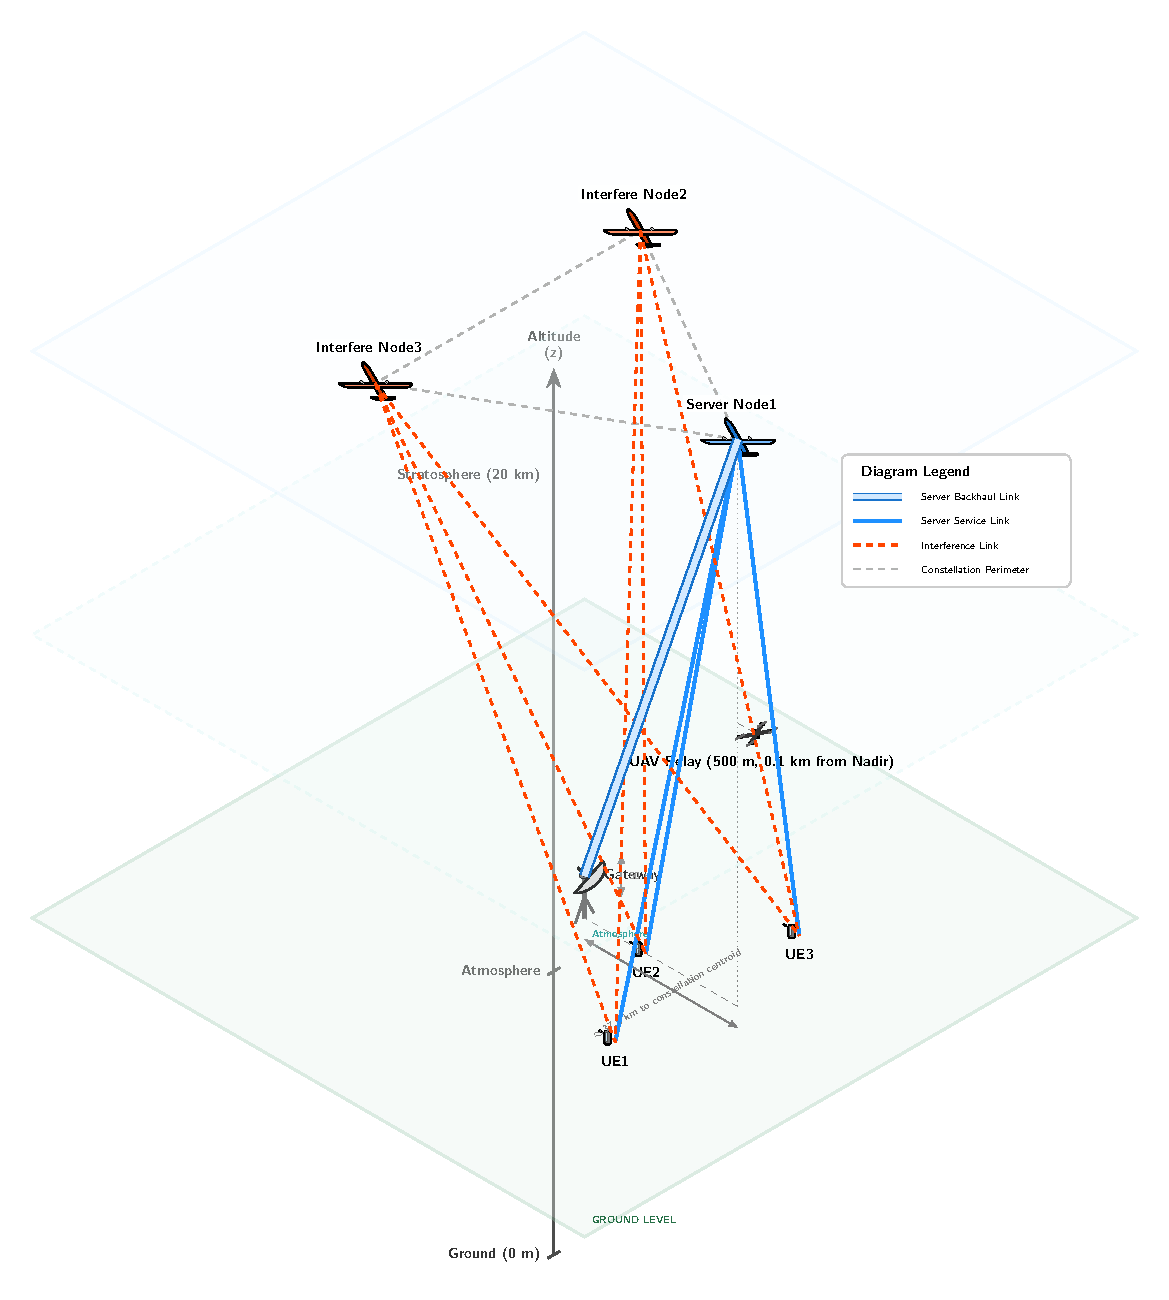
\includegraphics[width=0.72\linewidth]{./figures/network_diagram_gw.pdf}
\caption{Network topology: three HAPS nodes and one UAV relay serve ground users over an access layer; a single ground gateway aggregates the backhaul links into the core network.}
\label{fig:simulation-topology}
\end{figure}

\subsection{FSPL, Applicable to All Channels}

The ITU-R P.530 free-space path loss~\cite{itu_p530} is
\begin{equation}
L_\mathrm{FSPL} = 32.44 + 20\log_{10} f_\mathrm{MHz} + 20\log_{10} d_\mathrm{km} \;[\mathrm{dB}],
\label{eq:fspl}
\end{equation}
where $f_\mathrm{MHz}$ is the carrier frequency and $d_\mathrm{km}$ the link distance. This is algebraically the wavelength form $L_\mathrm{FSPL}(h,r)=20\log_{10}(4\pi d_{h,r}/\lambda)$ used later in the multi-HAPS SINR formulation (\S\ref{sec:multihaps}): substituting $\lambda=c/f$ and converting units folds the resulting constant into the $32.44$\,dB term above.

\begin{figure}[H]\centering
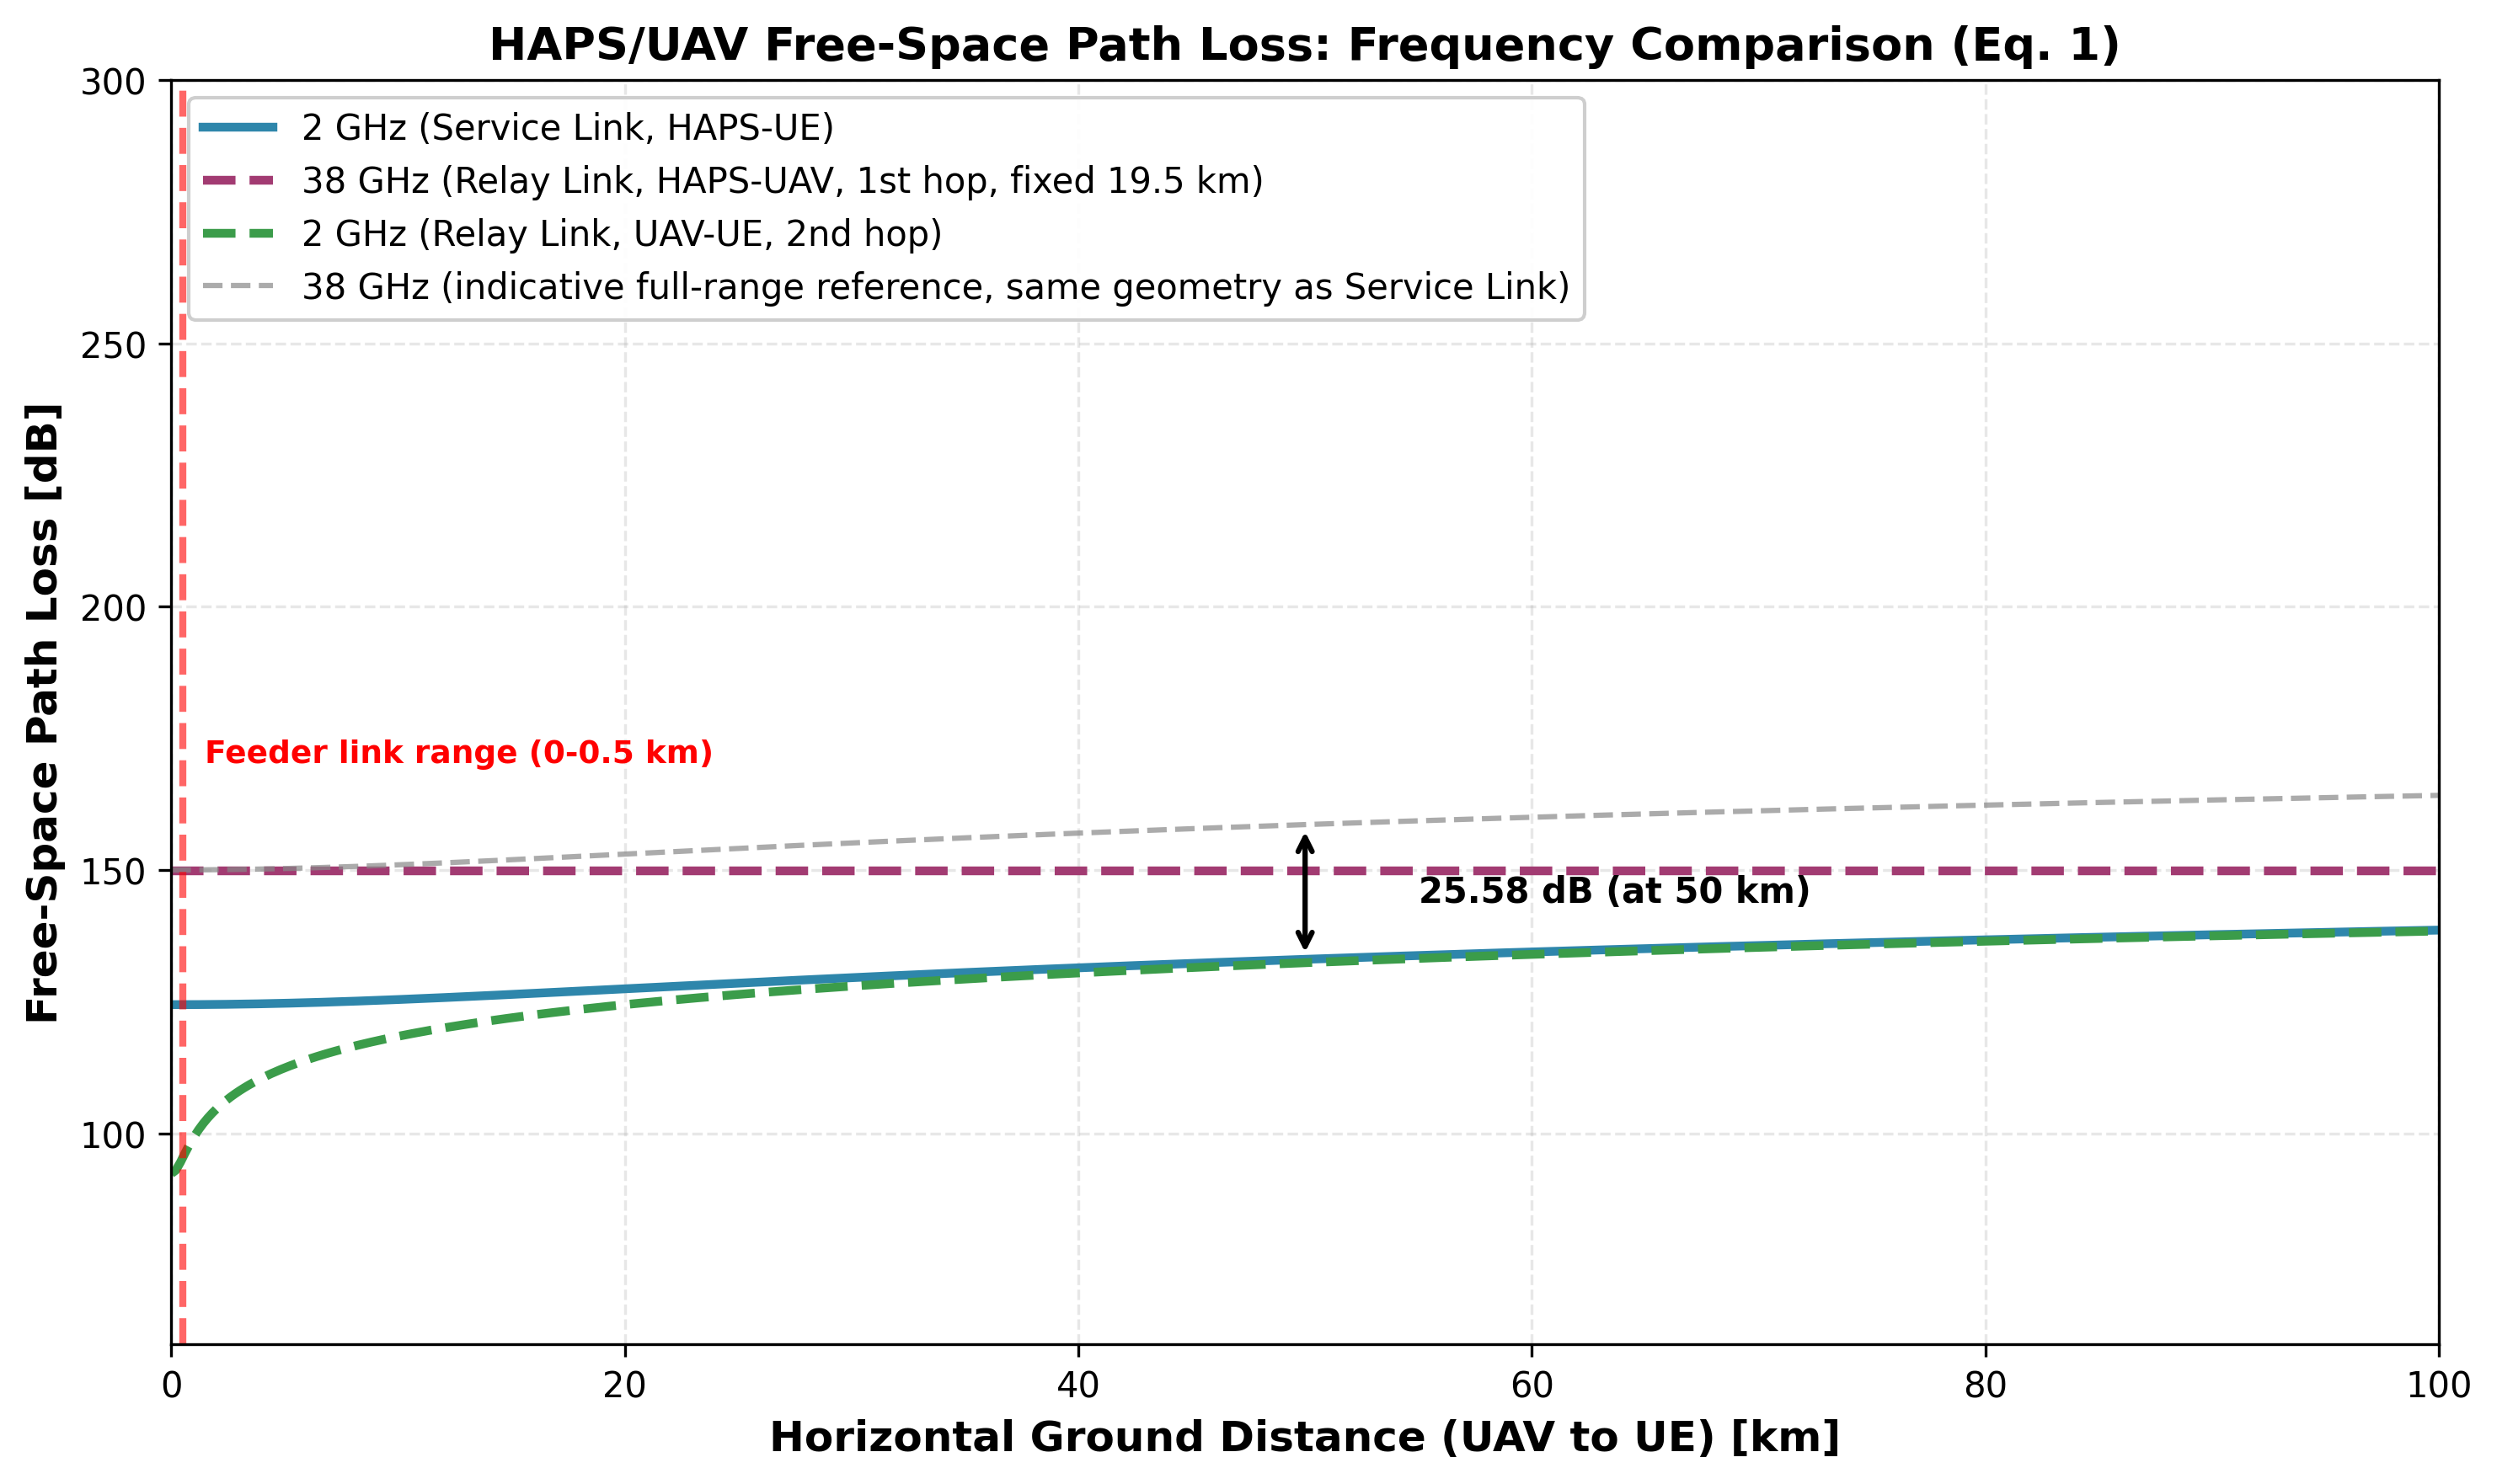
\includegraphics[width=0.95\columnwidth]{./figures/1b_haps_fspl_2ghz_vs_38ghz.png}
\caption{FSPL vs.\ distance (Eq.~\eqref{eq:fspl}) -- same functional form for 2 and 38~GHz; the 38~GHz feeder sits $\approx$25.6\,dB higher, purely from the $20\log_{10}(38/2)$ frequency term.}
\label{fig:fspl_comparison}
\end{figure}

\subsection{38.0~GHz Frequency Channels}
\label{subsec:backhaul-model}
\label{sec:channel-models}

\textbf{Rain Attenuation.} 
Rain attenuation $\gamma_R$ (dB/km) follows the ITU-R P.838 power law~\cite{itu_p838}
\begin{equation}
\gamma_R = k(f,\theta)\,R^{\alpha(f,\theta)} \quad [\mathrm{dB/km}],
\label{eq:rain_spec_atten}
\end{equation}

Total rain loss is using the ITU-R P.618 effective slant length $L_\mathrm{eff}$~\cite{itu_p618}
\begin{equation}
A_\mathrm{rain}=\gamma_R L_\mathrm{eff},
\label{eq:total_rain_loss}
\end{equation}

\textbf{Atmospheric Losses.}
Following are atmospheric losses that are modeled as specific attenuations times slant length:
Fog/cloud loss (ITU-R P.840~\cite{itu_p840}):
 $A_\mathrm{cloud}=\gamma_c(f,M,T)L_\mathrm{slant}$
Gas absorption (ITU-R P.676~\cite{itu_p676})
 $A_\mathrm{gas}=(\gamma_o+\gamma_w)L_\mathrm{slant}$;

\textbf{ Tropospheric scintillation}
Tropospheric scintillation  (ITU-R P.618 Annex~1~\cite{itu_p618}) is given by 
\begin{equation}
A_\mathrm{scint}(p) = a(p)\cdot\sigma_\mathrm{pre}(f,\theta,\mathrm{climate}) \quad [\mathrm{dB}],
\label{eq:scint_loss}
\end{equation}
growing with frequency and shrinking with elevation.

Total 38.0 Ghz backhaul/feeder slant-path attenuation sums all terms:
\begin{equation}
L_\mathrm{total} = L_\mathrm{FSPL} + A_\mathrm{rain} + A_\mathrm{cloud/fog} + A_\mathrm{gas} + A_\mathrm{scint}.
\label{eq:feeder_loss}
\end{equation}

\subsection{2~GHz Service/Relay Link}
\label{subsec:service-model}

\textbf{Building Blockage.} For a UAV or HAPS node $u$ at horizontal distance $r_{u,k}$ from user $k$, the Line-of-Sight (LoS) probability follows the building-blockage product series of Arani et al.~\cite{arani2023}, parameterised by Holis \& Pechac~\cite{holispechac2008}:
\begin{equation}
P^\mathrm{LoS}_{u,k} = \prod_{n=0}^{J}\left[1-\exp\!\left(-\frac{1}{2\xi^2}\Big(h_u-\tfrac{n+\frac12}{J+1}(h_u-h_k)\Big)^{2}\right)\right],
\label{eq:los}
\end{equation}
with $J=\lfloor \tfrac{r_{u,k}}{1000}\sqrt{\alpha\beta}-1\rfloor$ building layers, and environment-dependent parameters $(\alpha,\beta,\xi)$ (e.g.\ suburban $0.1,750,8$\,m; urban $0.3,500,15$\,m; dense urban $0.5,300,20$\,m; high-rise $0.5,300,50$\,m)~\cite{holispechac2008}.

Each propagation state $z\in\{\mathrm{LoS,NLoS}\}$ (LoS or Non-Line-of-Sight, NLoS) adds a log-normal shadowing term, averaged in linear gain (not dB, since the two states can differ by up to $\sim$17\,dB in dB-domain averaging):
\begin{align}
\overline{g} &= 10^{-\mathrm{FSPL}/10}\Big[P_\mathrm{LoS}\,e^{\tfrac{(a\sigma_\mathrm{LoS})^2}{2}} + P_\mathrm{NLoS}\,e^{-a\mu(\theta)+\tfrac{(a\sigma(\theta))^2}{2}}\Big],\nonumber\\
\overline{\mathrm{PL}} &= -10\log_{10}\overline{g}, \qquad a=\tfrac{\ln 10}{10}.
\label{eq:pl}
\end{align}
The downlink SINR at user $k$ from node $u$ is then
\begin{equation}
\gamma_{u,k} = \frac{p_u\,g_{u,k}}{\sum_{u'\neq u} p_{u'} g_{u',k} + \sigma_0^2}, \qquad g_{u,k}=10^{-\overline{\mathrm{PL}}/10}.
\label{eq:sinr}
\end{equation}

\subsection{Interference Model}
\label{sec:multihaps}

With three HAPS sharing spectrum, a serving HAPS $h$ provides the desired signal while the other two contribute co-channel interference at the same receiver $r$ (gateway, UAV, or UE):
\begin{equation}
\gamma_{h,r}=\frac{P_hG_hG_r g_{h,r}}{N_r + \displaystyle\sum_{h'\neq h}P_{h'}G_{h'}G_r g_{h',r}},
\label{eq:general-haps-sinr}
\end{equation}
with channel gain $g_{h,r}=10^{-L_{h,r}^\mathrm{tot}/10}$ from the total propagation loss of \S\ref{sec:channel-models}.

% =====================================================================
\section{Model Simulation and Results}
\label{sec:results}
% =====================================================================

We simulate the closed-form models above using a Python simulation stack (\texttt{NumPy}, \texttt{pandas}, \texttt{Matplotlib}); atmospheric and scintillation losses use the ITU-Rpy (\texttt{itur}) library's implementation of the relevant ITU-R recommendations. Following are the results of this simulation:

\subsection{Validating 38~GHz Choice Through Simulation}

This addresses a natural reader question: why not simply pick a lower-loss frequency instead of designing around rain, fog, and gas attenuation at 38~GHz?

\begin{figure}[H]\centering
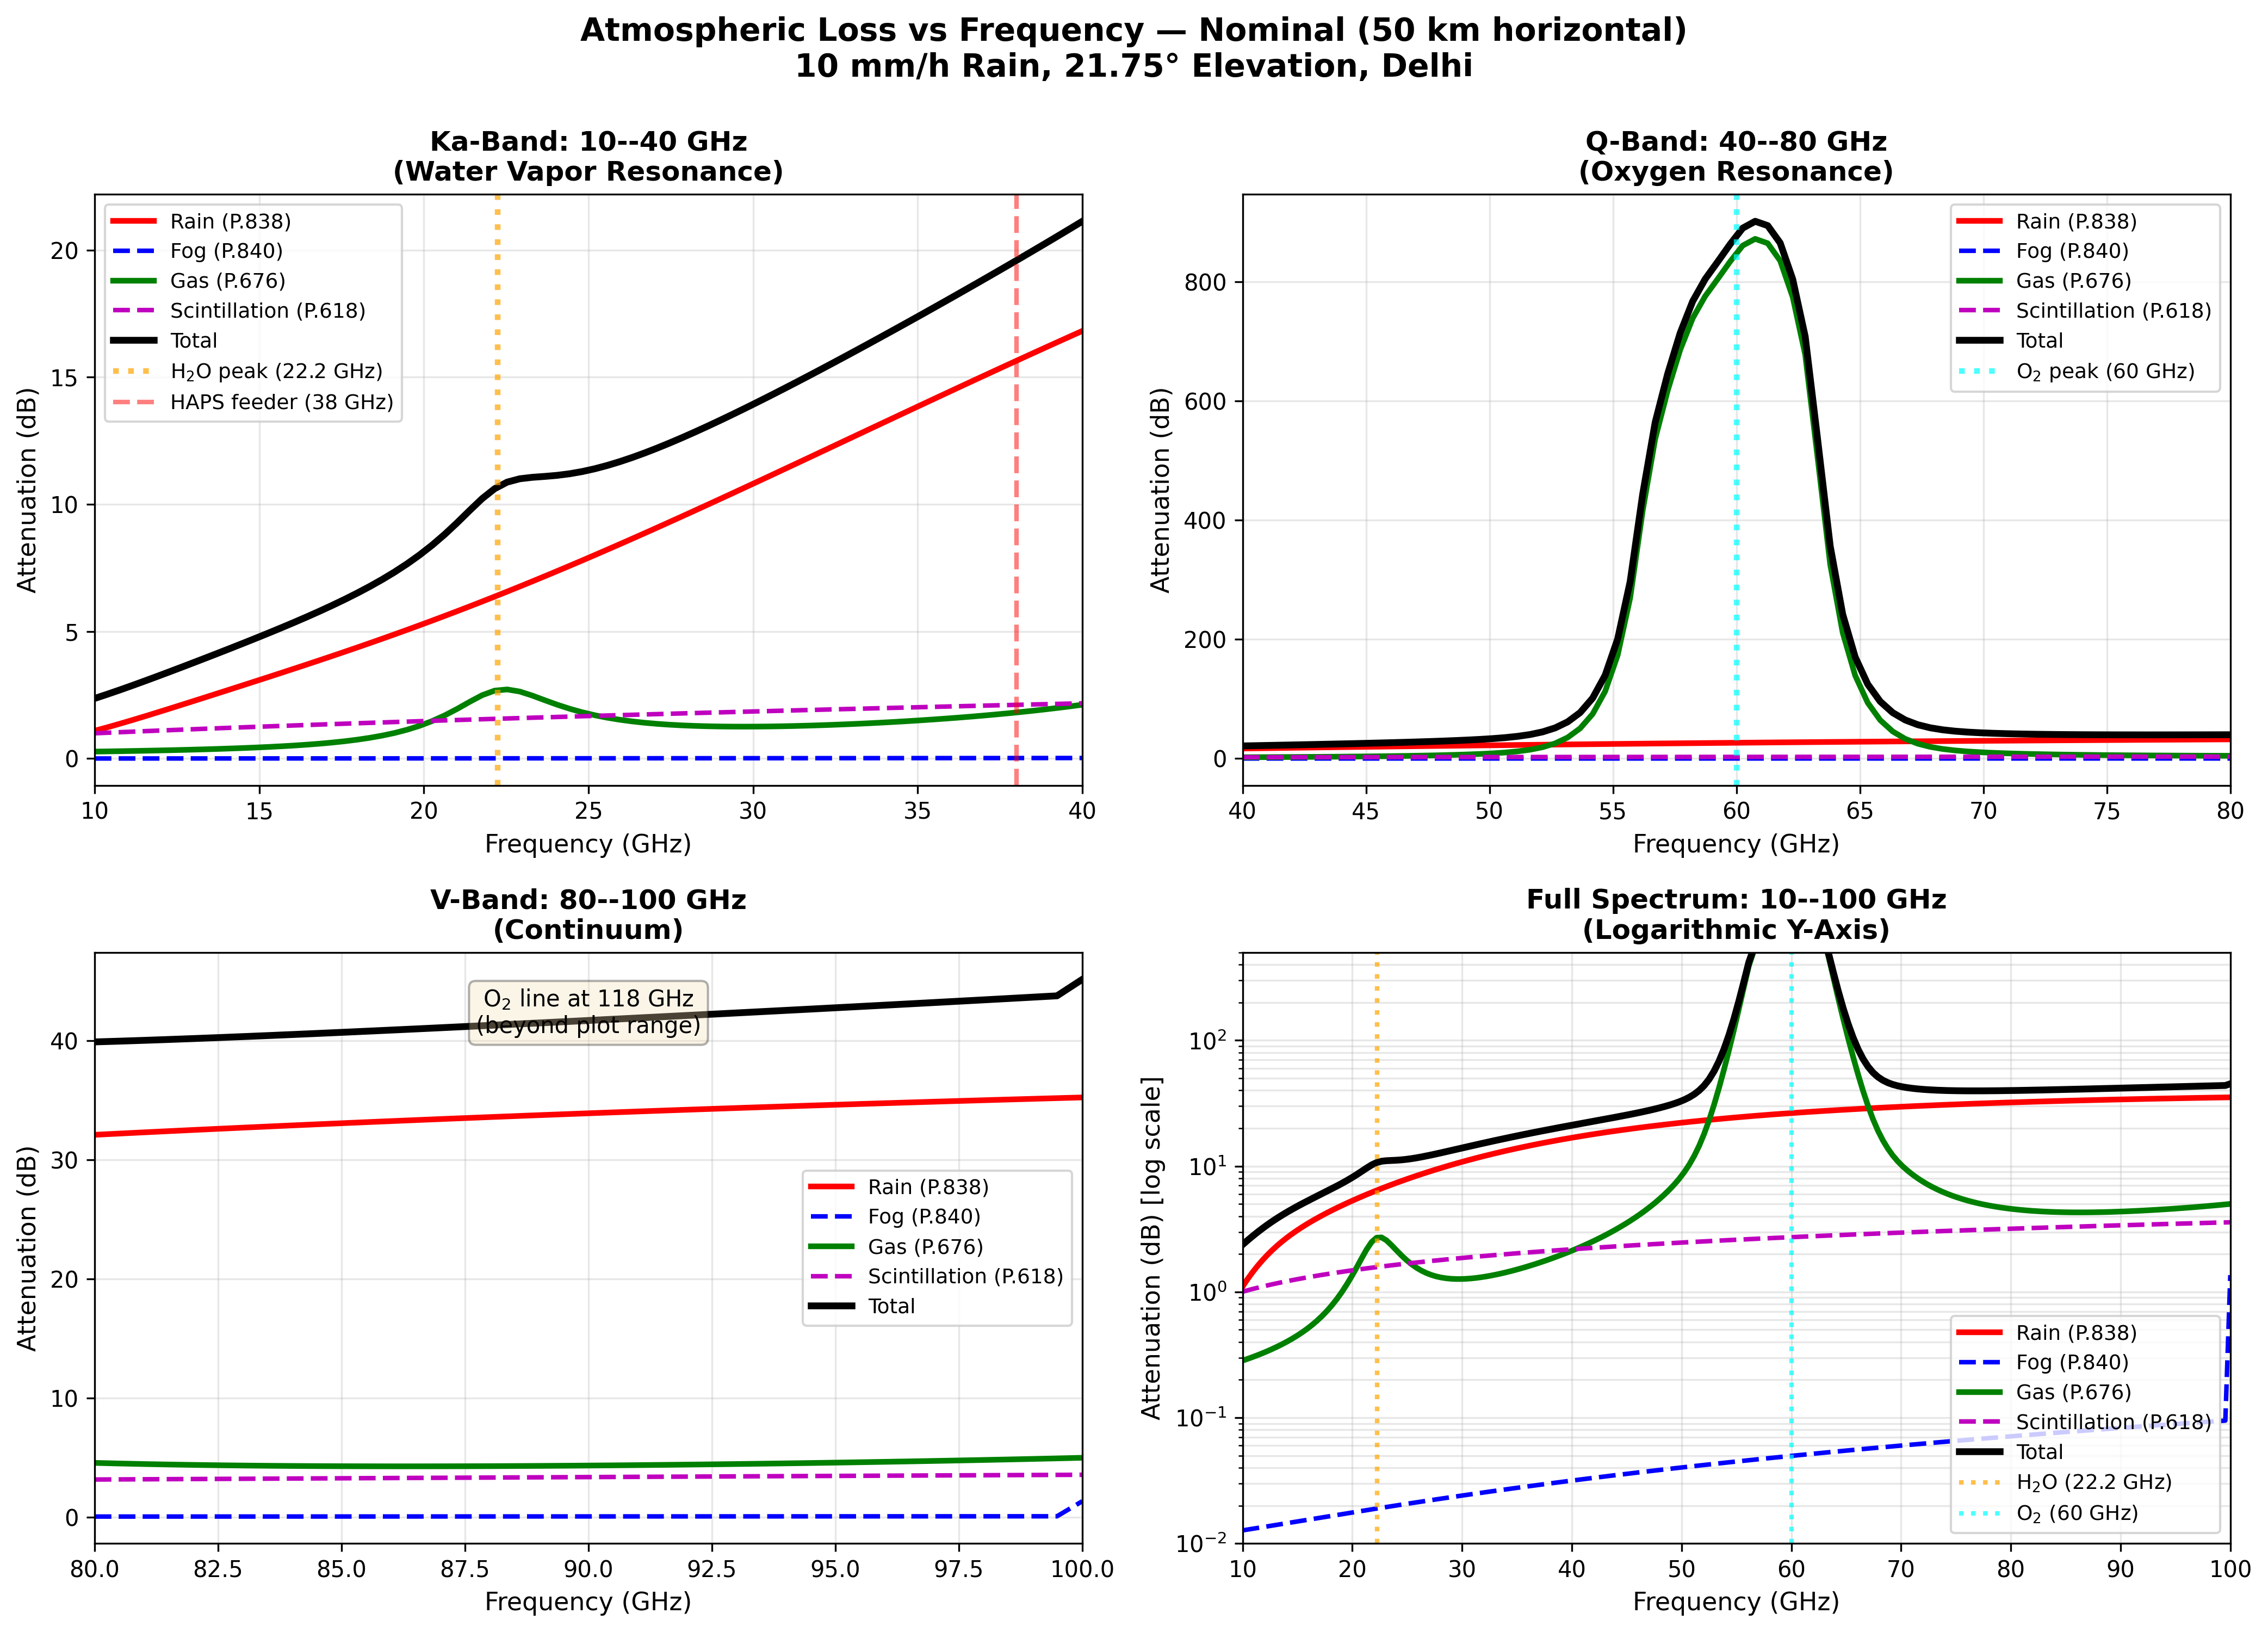
\includegraphics[width=0.95\columnwidth]{./figures/fig_atm_loss_nominal_frequency.png}
\caption{Atmospheric loss (rain, fog, gas) vs.\ frequency across the Ka/Q/V bands for the Delhi gateway path at 10\,mm/h rain.}
\label{fig:atm_frequency_nominal}
\end{figure}

From Fig.~\ref{fig:atm_frequency_nominal} we can notice that gas absorption (ITU-R P.676~\cite{itu_p676}) has two resonance peaks to avoid; frequency selection should avoid these. We also need higher frequencies to allow higher data aggregation. 

We also notice that at 38~GHz, both the fog/cloud and gas-absorption terms are small over the backhaul/feeder slant length: fog loss totals $<0.2$\,dB, and gas loss totals $\approx0.4$\,dB, since 38~GHz sits away from the gas-absorption resonance peaks.

Considering these factors, we validate the choice of 38.0~GHz range for HAPS (WRC-19).

\subsection{Analysing Rain Attenuation Through Simulation}

The simulated model is based on Delhi,  the backhaul/feeder margin  is evaluated at Delhi's rain statistics (ITU-R P.837), consistent with the 15--25\,dB Ka-band rain margins ECC Report 156~\cite{ecc_report_156} reports for Fixed Satellite Service (FSS) links -- a fair comparison, since FSS margins are derived for point-to-point links between two fixed terminals, which is exactly the geometry of our backhaul (Gateway fixed at the HAPS triangle's centroid) and feeder (UAV fixed 0.1\,km from the serving HAPS's own nadir) links, both evaluated at a constant elevation rather than a moving one. 

Link Margin which is the difference between the received signal strength and the atmospheric losses is evaluated as follows:
\begin{itemize}
  \item For 99.9\,\% availability, $R_{0.1}=15.7$\,mm/h, which gives $A_\mathrm{rain}\approx8.6$\,dB on the Gateway's centroid path, and $A_\mathrm{rain}\approx16.6$\,dB on the feeder's own near-zenith path.
  \item Backhaul SINR (FSPL and co-channel interference only, no atmospheric loss) is $\approx+39.9$\,dB, as per Eq.~\eqref{eq:general-haps-sinr} evaluated with $P_h=43$\,dBm, $G_h=13.8$\,dBi, and Gateway receive gain $G_g=39.7$\,dBi~\cite{karaman2025haps}, with $\approx0.4$\,dB of additional gas loss. Resulting link margin: $39.9-8.6-0.4\approx30.9$\,dB at 99.9\,\% availability.
  \item Feeder SINR (FSPL and co-channel interference only, no atmospheric loss) is $\approx+37.6$\,dB, as per Eq.~\eqref{eq:general-haps-sinr} evaluated with $P_h=43$\,dBm, $G_h=13.8$\,dBi, and UAV feeder-port receive gain $G_u=30.7$\,dBi~\cite{anim2021uav}, with $\approx0.4$\,dB of additional gas loss. Resulting link margin: $37.6-16.6-0.4\approx20.6$\,dB at 99.9\,\% availability.
\end{itemize}
 
This margin means link budget is sufficient to cover rain attenuation, even though the 38~GHz backhaul/feeder links are rain-dominated.


\begin{figure}[H]\centering
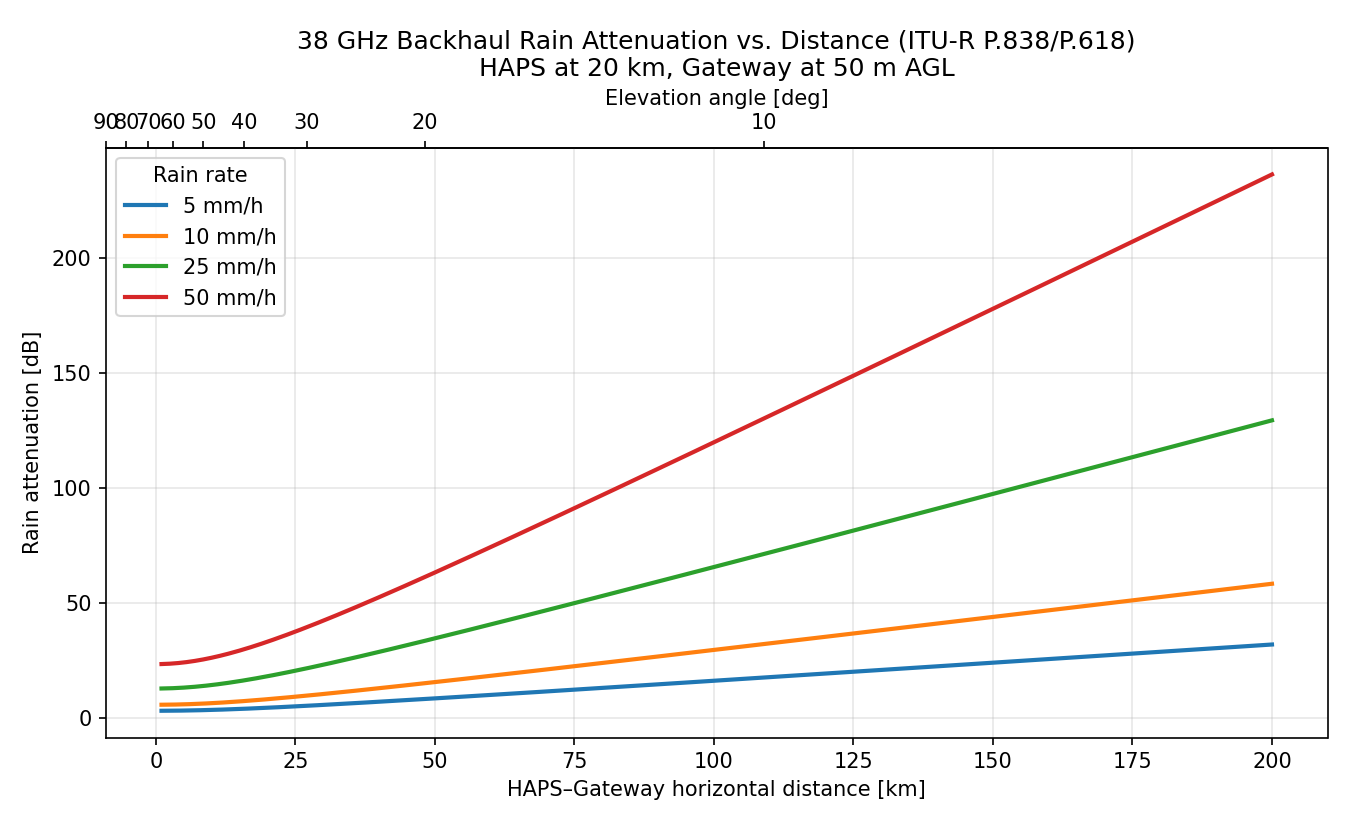
\includegraphics[width=0.95\columnwidth]{./figures/rain_attenuation_vs_distance.png}
\caption{38~GHz backhaul rain attenuation vs.\ HAPS--Gateway horizontal distance (ITU-R P.838/P.618), grows faster than linear past $\approx$100\,km as elevation drops and the slant path lengthens (\S\ref{subsec:backhaul-model}).}
\label{fig:rain-vs-distance}
\end{figure}

Though the backhaul/feeder links have sufficient margin to cover rain attenuation, the attenuation is still significant and time-varying, and is expected to become a greater concern if the number of UAVs is increased, since each additional UAV's feeder beam would then draw on the same HAPS transmit-power/capacity budget ($P_h$).

\subsection{Analysing Multi-HAPS Interference Through Simulation}


\begin{figure}[H]\centering
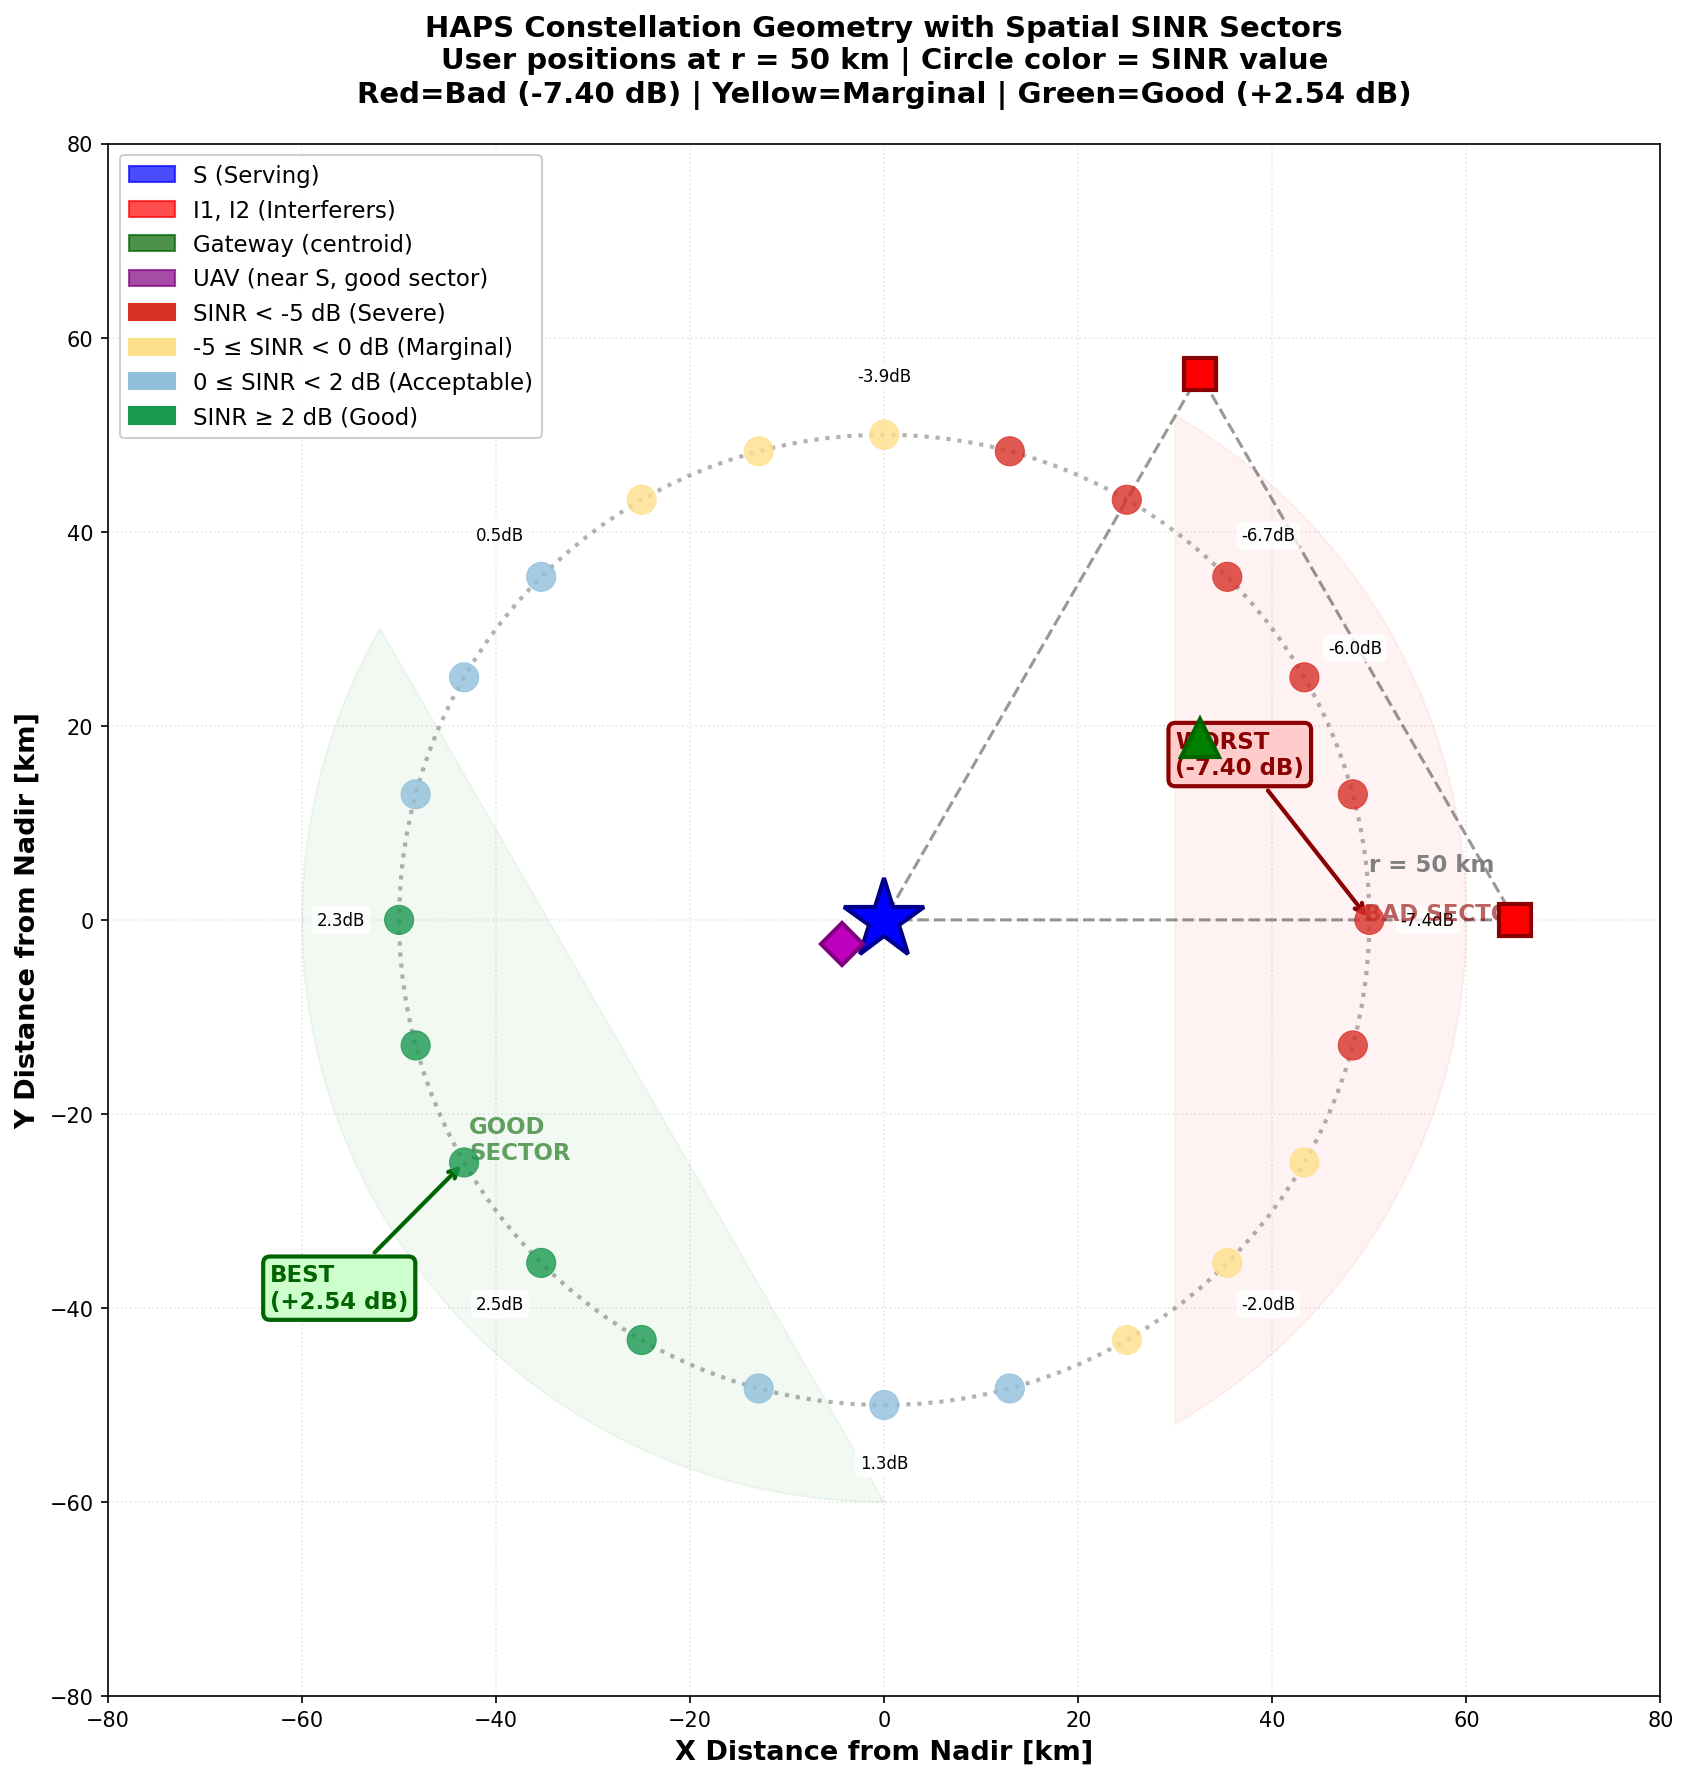
\includegraphics[width=0.68\columnwidth]{./figures/constellation_with_sectors.png}
\caption{HAPS constellation geometry (65\,km equilateral triangle: S at origin, I1 at $0^\circ$, I2 at $60^\circ$) with spatial SINR sectors at $r=50$\,km. Good sector (green, $\sim$120--290$^\circ$) vs.\ bad sector (red, $\sim$330--75$^\circ$). Best $+2.54$\,dB at $210^\circ$; worst $-7.40$\,dB at $0^\circ$.}
\label{fig:app-constellation-sectors}
\end{figure}

\label{sec:spatial-sinr}

Simulating the interference model explained in \S\ref{sec:multihaps} resulted in a good/bad-sector split in the HAPS constellation, as shown in Fig.~\ref{fig:app-constellation-sectors}; this, along with the scintillation fade simulation (Eq.~\eqref{eq:scint_loss}), motivated placing the UAV relay near the serving HAPS's nadir in the current model.

This angular spread is substantial: at a fixed 50~km radius, SINR varies by up to 9.94\,dB with angular position (Fig.~\ref{fig:app-constellation-sectors}), versus only $\sim$2--3\,dB from doubling the link distance indicating that angular position affects SINR more than distance does.

\begin{figure}[H]\centering
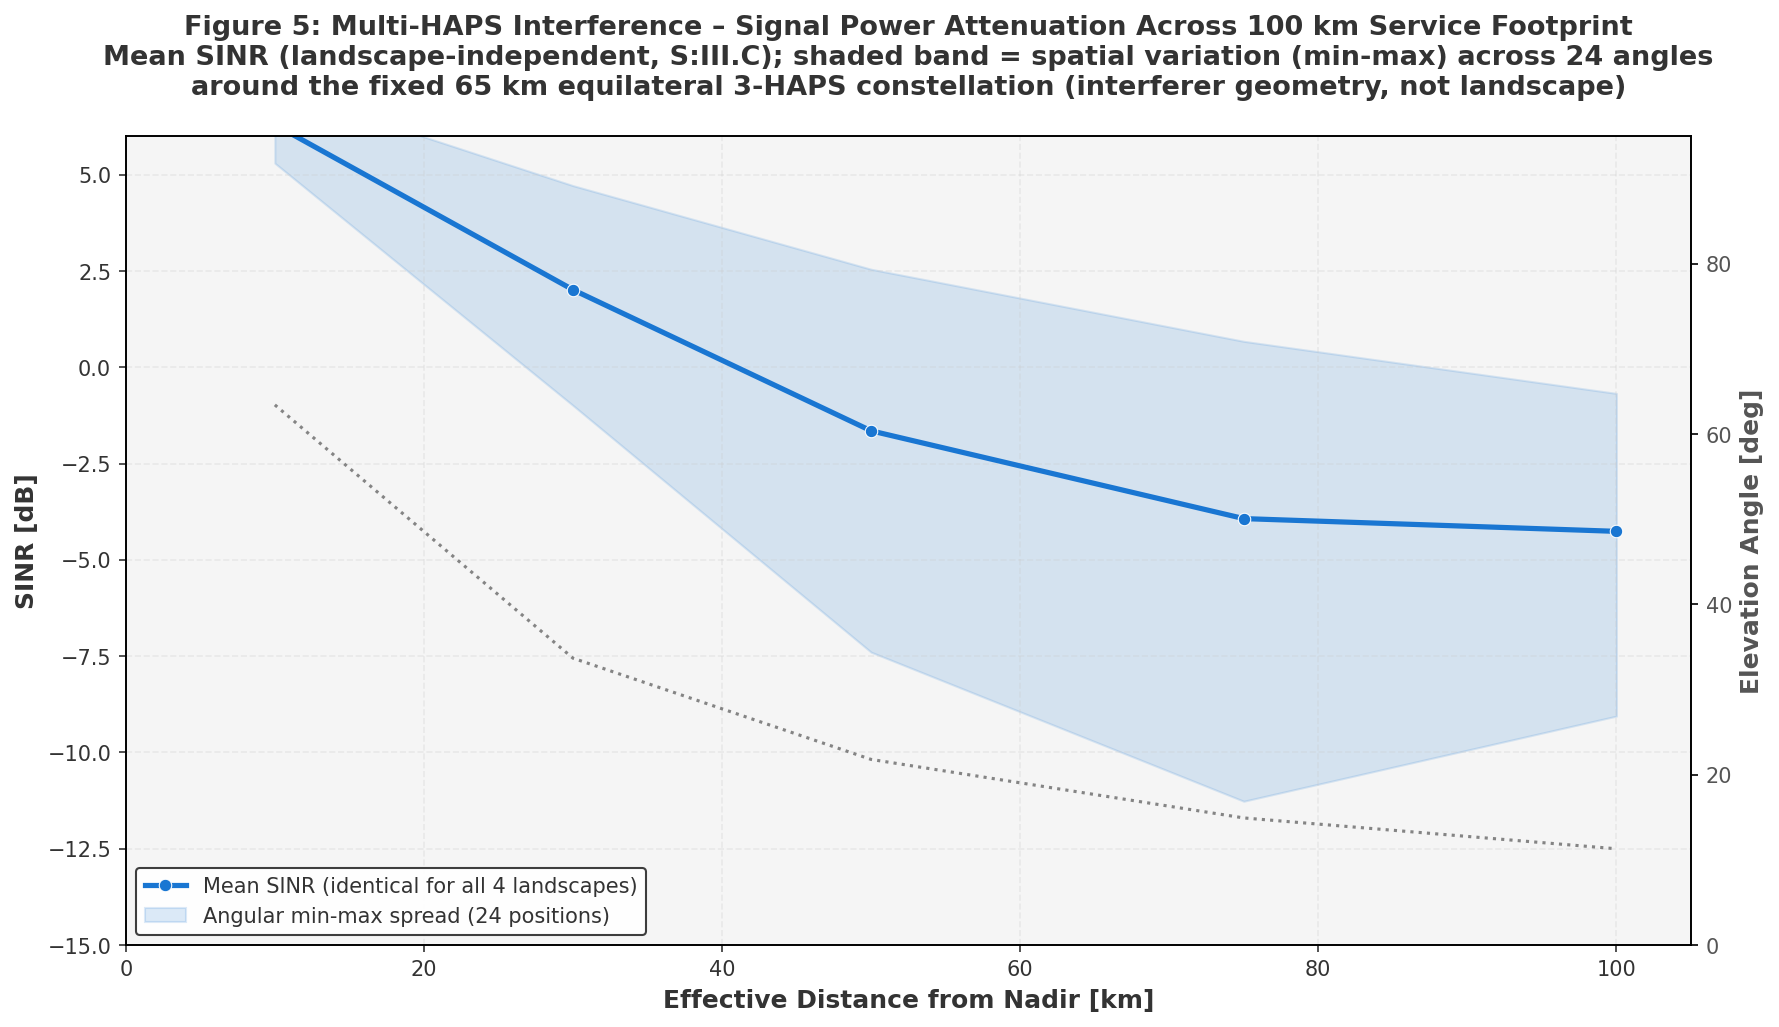
\includegraphics[width=0.95\columnwidth]{./figures/figure5_multi_haps_sinr_mean.png}
\caption{Mean SINR and angular min--max spread across the 100\,km service footprint: falls from $+6.3$\,dB at 10\,km to $-4.3$\,dB at 100\,km, while the spread widens to 11.94\,dB at 75\,km.}
\label{fig:multinode-interference}
\end{figure}

\subsection{Analysing Relay Path Behaviour Through Simulation}

Area-averaged capacity (bits/s/Hz) over disks of radius $R_\mathrm{eff}$ is the capacity considering no population or per-user sharing assumption (Monte Carlo average, $N=20{,}000$ uniform samples per disk).

We can observe that access hop (UAV$\to$UE, 2\,GHz) capacity drops with distance, collapsing far faster than the direct HAPS$\to$UE link because of low elevation. This allows us to compute a usable relay radius where access-hop capacity crosses a $0.5$\,bits/s/Hz floor, which is $R_\mathrm{eff}\approx6.5$\,km in urban terrain and $\approx10.3$\,km in suburban terrain (\S\ref{subsec:service-model}).

Within this effective radius the area-averaged capacity of different links is as in Table~\ref{tab:same-patch-ase}.

\begin{minipage}{\columnwidth}
\begin{center}
\footnotesize
\captionof{table}{Area-averaged capacity (bits/s/Hz) over disks of radius $R_\mathrm{eff}$}
\label{tab:same-patch-ase}
\begin{tabularx}{\columnwidth}{|>{\centering\arraybackslash}X|>{\centering\arraybackslash}X|>{\centering\arraybackslash}X|>{\centering\arraybackslash}X|>{\centering\arraybackslash}X|}
\hline
\textbf{Landscape} & \textbf{$R_\mathrm{eff}$ (km)} & \textbf{Direct @ HAPS nadir} & \textbf{Direct @ UAV's area} & \textbf{Access hop @ UAV} \\
\hline
Urban & 6.50 & 2.60 & 2.61 & 2.06 \\
\hline
Suburban & 10.31 & 2.52 & 2.52 & 2.19 \\
\hline
\end{tabularx}
\end{center}
\end{minipage}

\vspace{0.5em}
With uniform population distribution, 100\,km radius HAPS coverage area and our 3-HAPS geometry, a single HAPS's direct-link population is $(100^2/3)$ and a UAV's relay population is $R_\mathrm{eff}^2$, giving a user ratio of 79:1 in urban terrain and 31:1 in suburban terrain. At the edge of $R_\mathrm{eff}$, the relay's raw capacity drops to $\approx0.50$\,bits/s/Hz in both terrains, versus the direct link's area-averaged $2.60$\,bits/s/Hz (urban) and $2.52$\,bits/s/Hz (suburban) from Table~\ref{tab:same-patch-ase}. Dividing by the population ratio, the relay's per-user share at the edge is $15\times$ better in urban terrain ($0.50$ vs.\ $2.60/79=0.033$) and $6\times$ better in suburban terrain ($0.50$ vs.\ $2.52/31=0.081$); closer to the UAV, the relay wins by more.

Relay beats direct everywhere inside $R_\mathrm{eff}$.

The relay therefore helps every user within $R_\mathrm{eff}$ of the one fixed UAV, not the whole footprint -- a single static platform cannot be close to everyone across a 100\,km-radius footprint; \S\ref{sec:roadmap} quantifies how many additional, well-placed UAVs this implies. This motivates including the UAV relay as an association option for the learned policy of \S\ref{sec:dqn}, which (\S\ref{sec:dqn-results}) learns to invoke it for users it helps.


\subsection{Takeaway from Simulation Results}
\label{sec:motivation-learning}

A simple rule-based policy cannot account for three separate sources of variation this paper's channel and platform models expose, each of which a static or myopic rule handles poorly:
\begin{itemize}
  \item \emph{Spatial SINR heterogeneity.} Angular position relative to the two interfering HAPS affects SINR more than distance does (\S\ref{sec:spatial-sinr}), a pattern a simple ``always pick max-SINR'' rule cannot anticipate as a user moves.
  \item \emph{Time-varying weather.} Feeder-link rain attenuation changes hour to hour and must be anticipated, not just reacted to, since the agent must choose an association before that hour's rain is observed. \S\ref{sec:lstm} builds a forecaster for this.
  \item \emph{Battery depletion.} Each HAPS's state of charge depends on its load history, so a policy must balance load across platforms over time to avoid over-draining any one HAPS (\S\ref{subsec:battery}).
\end{itemize}
A learned, real-time association policy can condition on all three jointly, which is what the remainder of this part develops.

% =====================================================================
% =====================================================================
\section{Learned, Real-Time Association Policy for HAPS Selection}
% =====================================================================

\subsection{Baseline Association Policies}
\label{sec:baseline-policies}

As a control and basis for a learned policy, we evaluate three rule-based (non-learned) association policies on the above channel model. The choice for association for $N$ users is one of six options every hour: a direct link to HAPS1--3, or a UAV relay via HAPS1--3.

\begin{itemize}\setlength{\itemsep}{1pt}
  \item \textbf{Random}: uniform-random choice among the six options each hour (sanity floor).
  \item \textbf{Max-SINR}: always the best-SINR \emph{direct} link (Eq.~\eqref{eq:sinr}).
  \item \textbf{Max-throughput}: the highest-throughput option among all six every hour.
\end{itemize}

However it should be noted that Max-SINR needs evaluating the SINR of all three HAPS$\to$UE links, switching to each one in sequence, and doing this periodically to stay real-time -- rendering it a theoretical alternative rather than a deployable policy. Max-throughput, choosing among all six HAPS$\to$UE and relay options, assumes perfect, instantaneous knowledge of every option's SINR and capacity -- a theoretical upper bound, not a deployable policy.

\subsection{LSTM Rain-Attenuation Forecaster}
\label{sec:lstm}

We plan to forecast the dominant atmospheric parameter -- rain attenuation -- through an LSTM, as decided in \S\ref{subsec:backhaul-model}. We use the weather input from hourly NASA POWER, METAR and ERA5 data for Delhi over 2023--2026. The input consists of temperature, humidity, pressure, wind, precipitation, cloud amount, visibility, rain/fog codes, cloud liquid water, and sine/cosine encodings of time-of-day and season. The LSTM maps the past 24 hours of weather to the next six hourly values of HAPS-to-gateway rain attenuation at 38~GHz and $27.995^\circ$ elevation (the Gateway is fixed at the HAPS triangle's centroid, 42.50\,km slant range from the serving HAPS). A forecast for hour $t$ is issued at $t-1$ and evaluated strictly out-of-sample (e.g.\ 2026 forecasts come from a model trained only on 2023--2025 data), with early-stopping at the epoch with the best validation RMSE on held-out 2025 data to avoid overfitting.

The result of the LSTM run, depicted in Fig.~\ref{fig:lstm-2026} and compared against persistence in Table~\ref{tab:lstm-2026}, shows that the LSTM predicts rain attenuation with lower RMSE than the persistence baseline at every horizon except $+1$\,h, where persistence has lower RMSE; at $+2$\,h persistence also has a narrowly lower MAE.

\begin{figure}[H]
\centering
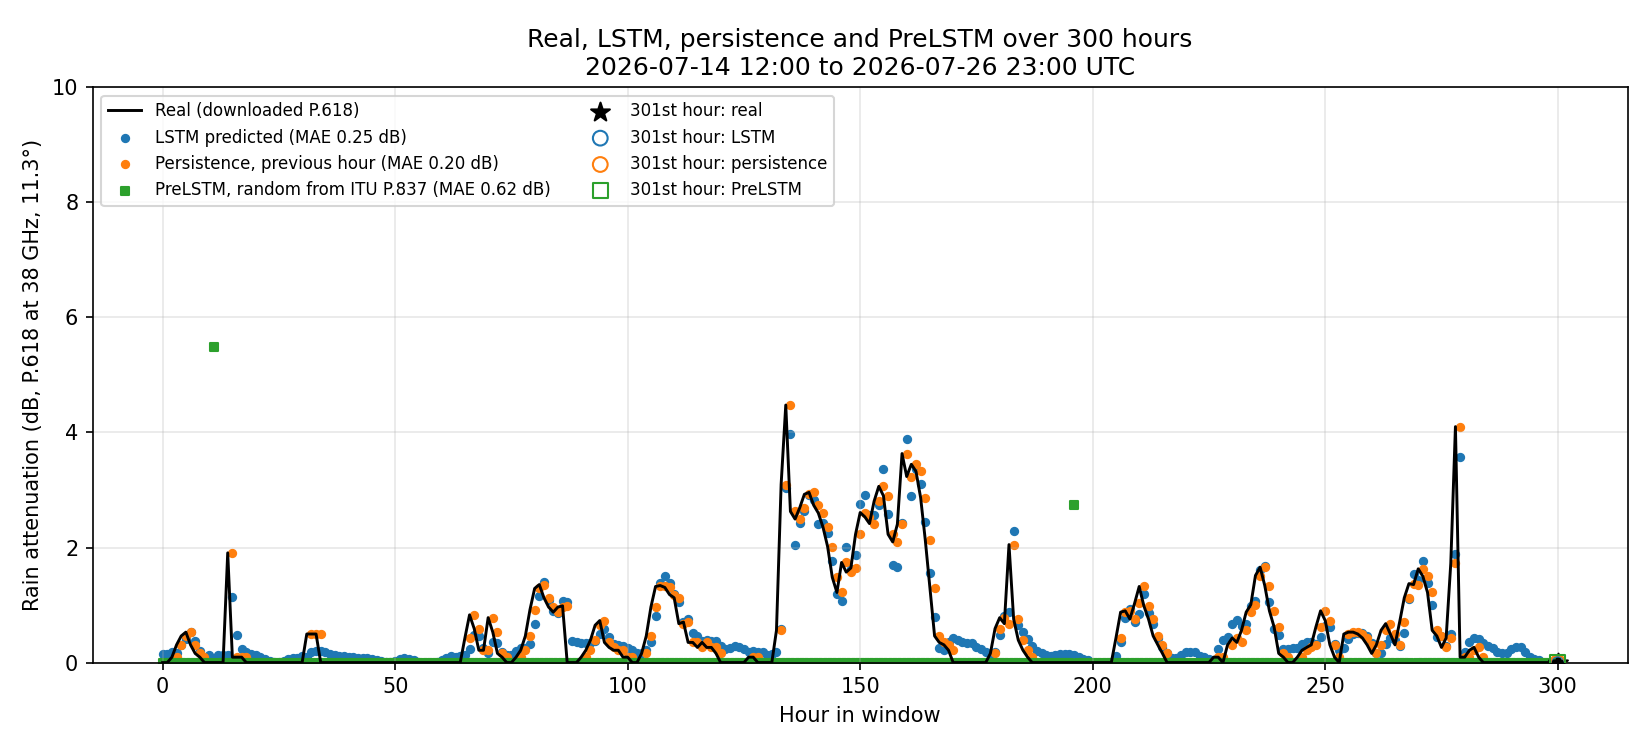
\includegraphics[width=\linewidth]{./figures/lstm_forecast_2026.png}
\caption{Real, LSTM, persistence and a synthetic PreLSTM baseline over a 300-hour window in July 2026 (the window with the most rain). LSTM: one-hour-ahead forecast. Persistence: previous hour's value. PreLSTM: random hourly rain rates drawn from ITU-R P.837 statistics, converted via P.618.}
\label{fig:lstm-2026}
\end{figure}

\begin{table}[H]
\centering
\caption{LSTM (early-stopped at the epoch validated on held-out 2025, \S\ref{sec:dqn-results}) against persistence on 2026 (6556 forecast hours, no 2026 data in training): MAE/RMSE in dB per horizon. Bold marks the better method.}
\label{tab:lstm-2026}
{\scriptsize\setlength{\tabcolsep}{3pt}
\begin{tabularx}{\columnwidth}{|>{\centering\arraybackslash}X|>{\centering\arraybackslash}X|>{\centering\arraybackslash}X|>{\centering\arraybackslash}X|>{\centering\arraybackslash}X|}
\hline
\textbf{Horizon} & \textbf{LSTM MAE} & \textbf{Persist.\ MAE} & \textbf{LSTM RMSE} & \textbf{Persist.\ RMSE} \\
\hline
$+1$\,h & $0.15$ & $\mathbf{0.12}$ & $0.54$ & $\mathbf{0.53}$ \\
\hline
$+2$\,h & $0.21$ & $\mathbf{0.20}$ & $\mathbf{0.70}$ & $0.75$ \\
\hline
$+3$\,h & $\mathbf{0.24}$ & $0.26$ & $\mathbf{0.80}$ & $0.90$ \\
\hline
$+4$\,h & $\mathbf{0.27}$ & $0.30$ & $\mathbf{0.86}$ & $1.02$ \\
\hline
$+5$\,h & $\mathbf{0.28}$ & $0.34$ & $\mathbf{0.90}$ & $1.11$ \\
\hline
$+6$\,h & $\mathbf{0.29}$ & $0.36$ & $\mathbf{0.92}$ & $1.17$ \\
\hline
\end{tabularx}}
\end{table}
\FloatBarrier

\subsection{DQN Association Agent}
\label{sec:dqn}

We choose DRL with a DQN to make the best association decision for HAPS. The following subsections detail the MDP formulation (state, action, and reward) and the battery model used.

\subsubsection{MDP Formulation}

\textbf{Number of MDPs.} The association problem decomposes into two MDPs, not one, both solved by the same DQN.

\emph{(1) An $N$-user MDP, for service/access-link association.} With $N$ users, a centralized MDP over joint assignments is intractable, so each user independently chooses a platform every hour, and reward is computed after all assignments.

\emph{(2) An $M$-UAV MDP ($M=1$ here), for feeder-link association.} The single, static relay UAV (Table~\ref{tab:config}) has one physical feeder radio, so which HAPS feeds it is a separate, per-UAV, per-hour decision, shared by every user who relays that hour -- not something any one user's own action can set. A fleet of $M$ UAVs would turn this into an $M$-UAV assignment problem (e.g.\ the $\sim$200-UAV deployment of \S\ref{sec:roadmap}); here $M=1$, so there is exactly one such decision per hour.

At each hour, the same DQN first chooses every user's action for the $N$-user MDP, then takes one extra forward pass on that hour's mean user state to greedily pick the feeder HAPS for the $M$-UAV MDP. Both choices are trained off the same replay buffer and repeat every hour across the episode. This single global mean does not scale to $M>1$ UAVs without a per-UAV context; nevertheless, it works for the current single-UAV geometry.

\textbf{MDP Parameters.} Each of the three HAPS platforms can serve a user directly, giving six actions $a_k\in\{0,\dots,5\}$ (actions 0--2: direct HAPS1--3; actions 3--5: relay via the UAV). The HAPS sub-index of a relay action is not used -- which HAPS the UAV's feeder actually binds to is decided separately, as above.

\textbf{State} (per user, 21-dimensional):
\begin{enumerate}\setlength{\itemsep}{1pt}
  \item SINR to each of the 3 platforms (dB, Eq.~\eqref{eq:sinr}) -- 3 dims
  \item horizontal distance to each of the 3 platforms (km) -- 3 dims
  \item each HAPS's battery state of charge (\%, \S\ref{subsec:battery}) -- 3 dims
  \item rainfall rate -- 1 dim
  \item visibility -- 1 dim
  \item time-of-day -- 1 dim
  \item UAV-relay capacity to each of the 3 platforms (bits/s/Hz) -- 3 dims
  \item the six LSTM rain forecasts $\hat{A}_t,\dots,\hat{A}_{t+5}$ (\S\ref{sec:lstm}), issued at $t-1$ so no rain of hour $t$ enters the state -- 6 dims
\end{enumerate}

\textbf{Reward and Penalty.} For user $k$ with linear SINR $\gamma_k=10^{\mathrm{SINR}_{k,\mathrm{dB}}/10}$ on its chosen link,
\begin{align}
r_k &= \omega_1 T_k c_\mathrm{rain} + P^\mathrm{sev}_k + P^\mathrm{deg}_k + \omega_2 J_\mathrm{fair} - \omega_3 P_\mathrm{eng} + P_\mathrm{LB},\nonumber\\
T_k &= \log_2(1+\gamma_k), \qquad c_\mathrm{rain}=10^{-A_\mathrm{rain}/10}\in[0.05,1],\nonumber\\
J_\mathrm{fair} &= \frac{(\sum_k\gamma_k)^2}{N\sum_k\gamma_k^2}, \qquad P_\mathrm{eng}=\frac{1}{3}\sum_{p=1}^3\Big(1-\frac{\mathrm{SoC}_p}{100}\Big),
\label{eq:reward}
\end{align}
with $\omega_1=0.5,\omega_2=0.3,\omega_3=0.2$; $c_\mathrm{rain}$ de-rates every user's throughput credit alike, whether served directly or via the UAV relay, because all traffic -- direct or relayed -- ultimately transits the rain-faded 38~GHz backhaul to reach the core network (\S\ref{sec:topology}). $c_\mathrm{rain}$ leaves the other reward terms (fairness, outage, energy) untouched. Penalties (per user): severe outage $P^\mathrm{sev}_k=-100$ if $\mathrm{SINR}_{k,\mathrm{dB}}<-2$\,dB; degraded service $P^\mathrm{deg}_k=-20$ if $-2\le\mathrm{SINR}_{k,\mathrm{dB}}<0$\,dB; and a shared low-battery penalty $P_\mathrm{LB}=-50$ for any platform with $\mathrm{SoC}_p<10\,\%$ and at least one assigned user. The reported fairness metric (Jain index~\cite{jain1984quantitative} over per-user delivered throughput, $T_kc_\mathrm{rain}$) differs from $J_\mathrm{fair}$ above, which is Jain over linear SINR and enters only the reward.

\subsubsection{Battery Model Coupled with DQN State and Reward}
\label{subsec:battery}

Battery state of charge enters the DQN in two places: as a per-platform state feature (\S\ref{sec:dqn}), and as the low-battery penalty $P_\mathrm{LB}$ above. The following describes how it evolves. Each HAPS's battery state of charge (SoC) is tracked hourly,
\begin{equation}
\Delta\mathrm{SoC} = \frac{P_\mathrm{solar}(t) - (P_\mathrm{backhaul}+P_\mathrm{payload}+\sum_k P_{k,\mathrm{user}})}{C_\mathrm{battery}},
\label{eq:battery-balance}
\end{equation}
with $P_\mathrm{backhaul}=500$\,W, $P_\mathrm{payload}=200$\,W, and $C_\mathrm{battery}=12\,000$\,Wh. Because the HAPS operates above $>$99\,\% of clouds, solar generation is independent of ground weather and follows a diurnal cosine profile,
\begin{equation}
I_0(t_\mathrm{hr}) = \begin{cases} 600\cos\!\big(\pi(t_\mathrm{hr}-12)/12\big) & 6\le t_\mathrm{hr}\le 18\\ 0 & \text{night}\end{cases}\ [\mathrm{W/m^2}],
\end{equation}
giving $P_\mathrm{solar}(t)=20\,\mathrm{m}^2\times0.20\times I_0(t)$, i.e.\ $2400$\,W at noon and $0$\,W at night. SoC is clipped to $[0,100]\,\%$; below $5\,\%$ the platform shuts down (no service), and below $10\,\%$ with assigned users the reward's low-battery penalty applies, so the agent must learn to balance load across platforms to avoid over-draining any one HAPS overnight.

\subsection{DQN Results}
\label{sec:dqn-results}

\begin{itemize}\setlength{\itemsep}{1pt}
  \item \textbf{Baselines.} Random, max-SINR, and max-throughput (\S\ref{sec:baseline-policies}) vs.\ the LSTM+DQN agent (\S\ref{sec:dqn}), all on the same held-out days and six-action set.
  \item \textbf{Implementation.} Custom PyTorch network (\texttt{torch}, \texttt{torch.nn}).
  \item \textbf{Input data.} 400 real 2024 episodes (weather-conditioned, \S\ref{sec:lstm}).
  \item \textbf{Training.} Rolling 24-hour episodes; 2400 episodes total, cycling the 400 real 2024 episodes six times.
  \item \textbf{Validation.} 50 held-out 2025 days, across ten seeded experiments with different random seeds.
  \item \textbf{Variants run.} Four policies (random, max-SINR, max-throughput, LSTM+DQN) plus three forecast ablations of the DQN itself (\texttt{lstm}, \texttt{none}, \texttt{oracle}), each under the same ten-seed protocol.
\end{itemize}

\begin{table}[H]
\centering
\caption{Policy comparison, 50 held-out 2025 days, mean over ten experiments (std.\ dev.\ across experiments in parentheses). Jain is over per-user delivered throughput.}
\label{tab:dqn-all-policies}
{\footnotesize\setlength{\tabcolsep}{4pt}\renewcommand{\arraystretch}{1.25}
\begin{tabularx}{\columnwidth}{|>{\raggedright\arraybackslash}p{0.30\columnwidth}|>{\centering\arraybackslash}X|>{\centering\arraybackslash}X|>{\centering\arraybackslash}X|}
\hline
\textbf{Policy} & \textbf{Reward/step} & \textbf{Jain} & \textbf{Outage/50} \\
\hline
Random (six actions) & $-92.2\,(1.4)$ & $0.255\,(0.011)$ & $41.6\,(0.3)$ \\
\hline
Max-SINR (direct only) & $-14.5\,(1.7)$ & $\mathbf{0.558}\,(0.013)$ & $\mathbf{0.8}\,(0.2)$ \\
\hline
Max-throughput (six actions) & $\mathbf{-14.6}\,(1.7)$ & $0.241\,(0.039)$ & $\mathbf{0.8}\,(0.2)$ \\
\hline
LSTM + DQN & $-15.1\,(1.7)$ & $0.351\,(0.112)$ & $1.2\,(0.2)$ \\
\hline
\end{tabularx}}
\end{table}

LSTM+DQN is slightly behind the max-SINR and max-throughput baselines on reward and outage (Table~\ref{tab:dqn-all-policies}), but fairer than max-throughput (Jain $0.351$ vs.\ $0.241$, higher on 8 of 10 seeds, $p=0.0153$) and less fair than max-SINR ($0.558$, every seed, $p=0.0003$).

\FloatBarrier
Figs.~\ref{fig:seed-stats} and~\ref{fig:paired-forest} present these as seeded-experiment results: the same ten-seed, 2400-episode training/evaluation protocol repeated independently ten times, not a single run, so that the spread shown is run-to-run robustness rather than one-off variance.

\vspace{0.5em}
\begin{minipage}{\columnwidth}
\begin{center}
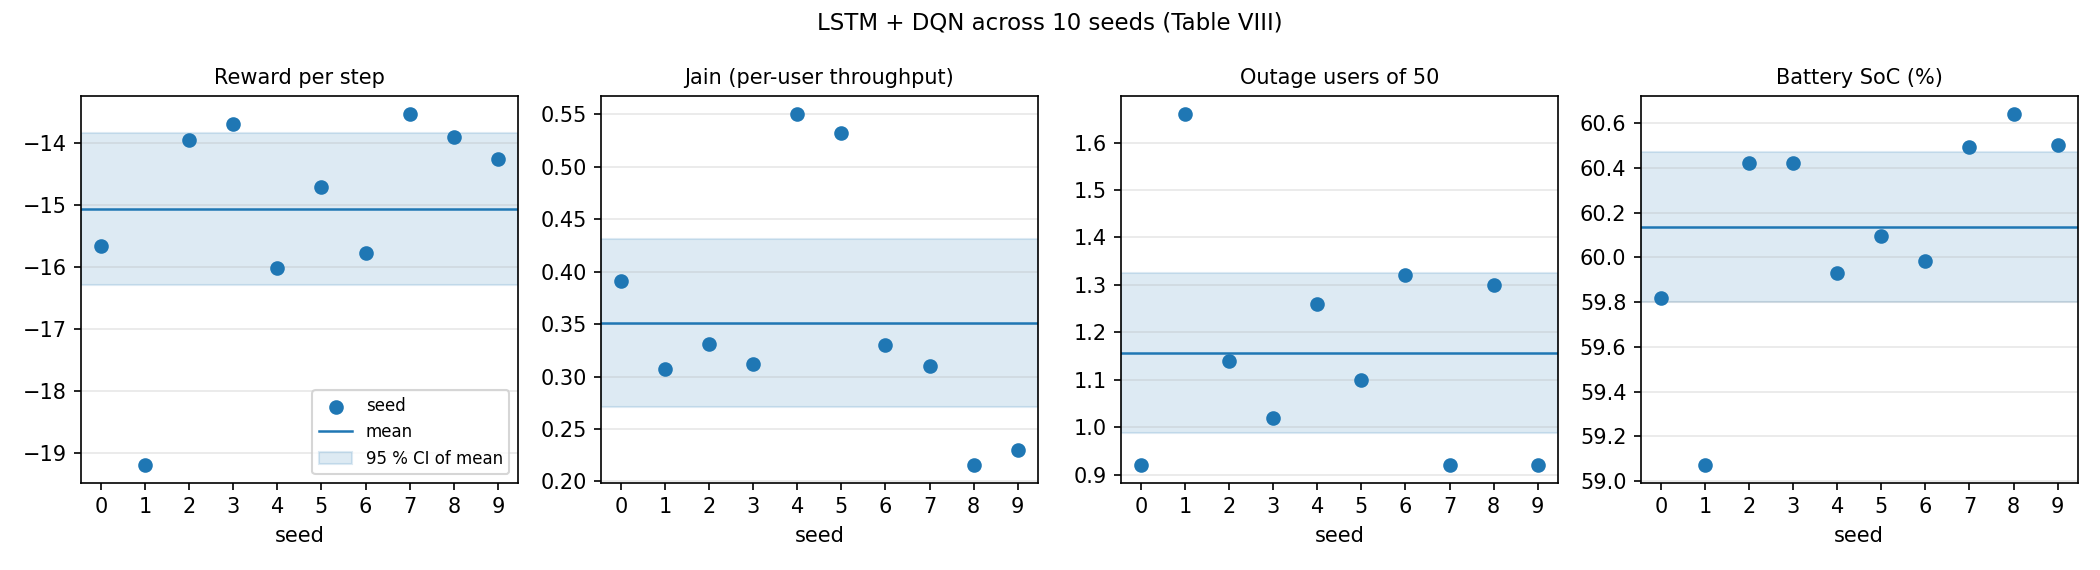
\includegraphics[width=\linewidth]{./figures/seed_stats.png}
\captionof{figure}{LSTM+DQN, ten independent seeds (dot = one training run; line = mean; band = 95\,\% CI of the mean).}
\label{fig:seed-stats}
\end{center}
\end{minipage}

\vspace{6pt}

Fig.~\ref{fig:seed-stats} reports reward, Jain fairness, outage, and battery SoC across the ten seeds; the shaded band reflects precision of the estimated mean, not run-to-run spread, so the tight spread shows the policy is reliably learned to this level, not a lucky or unlucky single run.

\begin{minipage}{\columnwidth}
\begin{center}
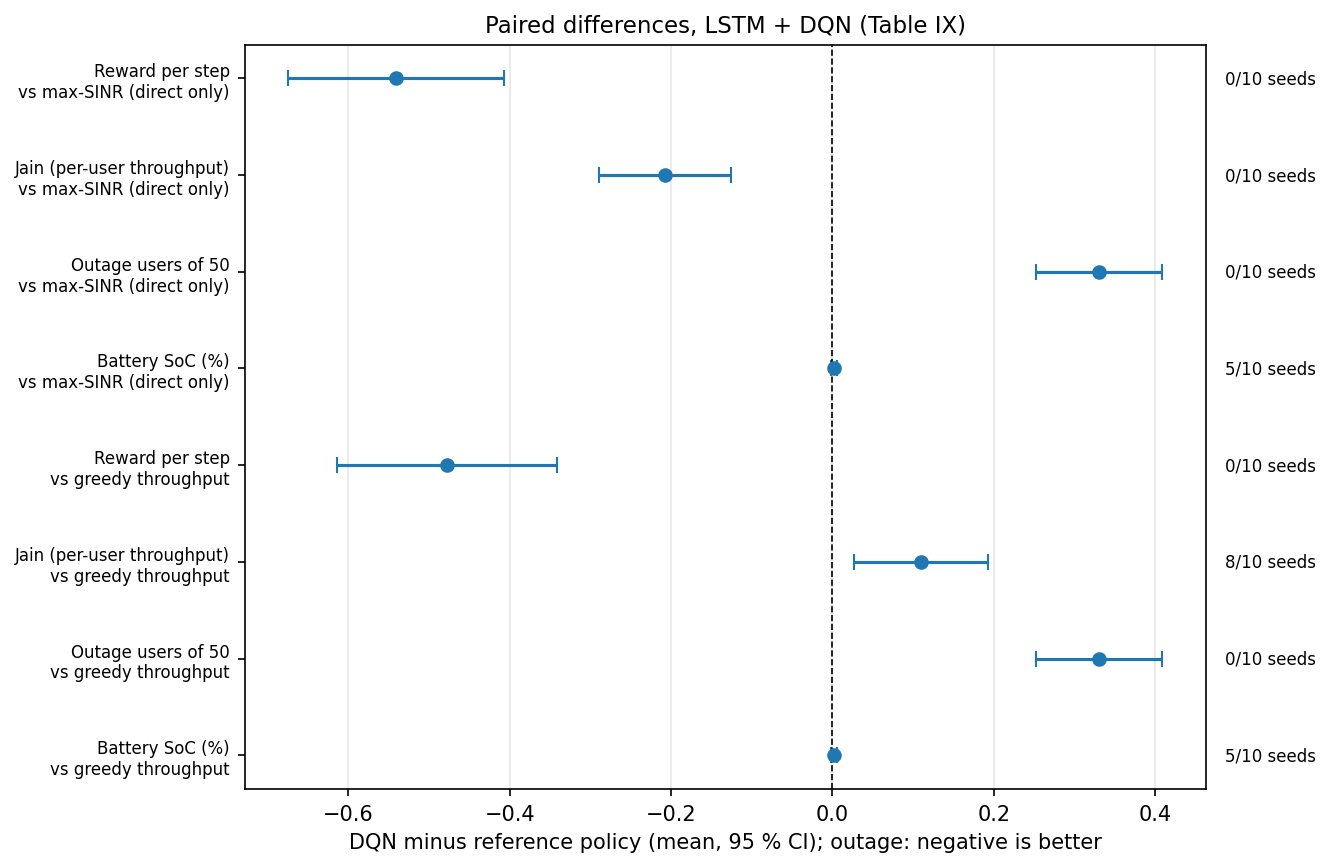
\includegraphics[width=0.8\linewidth]{./figures/paired_forest.png}
\captionof{figure}{Paired differences, LSTM+DQN minus baseline, per experiment (50 days, ten seeds); whiskers crossing zero are not significant.}
\label{fig:paired-forest}
\end{center}
\end{minipage}

\vspace{6pt}

\textbf{Summary of DQN results.}
\begin{itemize}\setlength{\itemsep}{2pt}
  \item \emph{Vs.\ baselines.} LSTM+DQN trails max-SINR and max-throughput on reward and outage on every seed; it is fairer than max-throughput on 8/10 seeds ($p=0.0153$) but less fair than max-SINR on every seed ($p=0.0003$).
  \item \emph{Operational cost of the baselines.} Max-SINR and max-throughput both need continuous, perfect, zero-latency measurement of every platform's SINR or capacity from every UE, an idealized assumption rather than something a real UE can actually provide; the DQN uses only its own locally available state.
  \item \emph{Impact of rain forecast.} Rain does not impact runs on this geometry, where the 2\,GHz access link and the margin-supported 38\,GHz feeder link both absorb it without needing to anticipate it. The forecaster's behaviour against persistence is nonetheless a useful input for more complex geometries where margins no longer absorb rain's losses and a forecast would actually matter.
  \item \emph{Deployability.} The DQN is the option that allows dynamic switching of links based on practical, learned-from-past-data behaviour, rather than the instantaneous, impractical periodic measurement of all available links that max-SINR and max-throughput require; at scale, with a UAV fleet covering the full 100\,km footprint (\S\ref{sec:roadmap}), the DQN becomes the inevitable option.
\end{itemize}
% =====================================================================
\section{Future Work}
\label{sec:roadmap}
% =====================================================================

\textbf{1) Model multiple UAVs.} The single, near-nadir UAV only covers its own $R_\mathrm{eff}$ disk (\S\ref{sec:results}), not the full footprint; gap-free coverage of the 100\,km service radius needs $\sim$200--270 such UAVs. This raises several new problems to solve:
\begin{itemize}\setlength{\itemsep}{1pt}
  \item \emph{UAV positioning.} Future work should let each UAV's altitude and horizontal distance adapt to user locations and to its distance from the serving HAPS, instead of the static, near-nadir placement used here.
  \item \emph{UAV-HAPS association.} The single-UAV, per-hour feeder-HAPS decision used here (\S\ref{sec:dqn}) should extend to $N$ UAVs and $M$ HAPS platforms, with feeder capacity contended across UAVs under the same HAPS.
  \item \emph{Cross-UAV interference and relative motion.} A fleet-scale model should add a UAV-to-UAV interference term to Eq.~\eqref{eq:general-haps-sinr} and model relative motion between HAPS platforms, UAVs, and users.
\end{itemize}

\textbf{2) LSTM and DQN improvements.} The forecast only pays off once a fleet lets several UAVs share one HAPS's feeder capacity, since only then can a forecast let the policy stagger reassignments ahead of a shared fade (\S\ref{sec:dqn-results}). Three directions follow from this:
\begin{itemize}\setlength{\itemsep}{1pt}
  \item \emph{Other impairments.} Future work should forecast fog liquid water content, scintillation, and gas absorption as time series, instead of treating them as instantaneous climatology values as done here.
  \item \emph{Feeder-context representation.} The DQN's feeder-HAPS choice should condition on a per-UAV, physically grounded representation of that UAV's own feeder channel, rather than the single global mean user state used here.
\end{itemize}

\textbf{3) Dynamic topology and geometry.}
\begin{itemize}\setlength{\itemsep}{1pt}
  \item \emph{Changing HAPS roles.} Shift a node between serving and interfering based on its distance to the gateway, and jointly optimize UAV/HAPS positioning across both roles a node could play at once, rather than each in isolation.
  \item \emph{Beamforming.} Consider beamforming between HAPS and gateway as geometry changes.
\end{itemize}

% =====================================================================
\section{Conclusion}
\label{sec:conclusion}
% =====================================================================

This document characterised the air-to-ground HAPS channels
across three link types -- the 2\,GHz HAPS$\rightarrow$UE service link,
the 38\,GHz HAPS$\rightarrow$Gateway backhaul link, and the two-hop
HAPS$\rightarrow$UAV$\rightarrow$UE relay link (whose first, 38\,GHz hop is
the feeder link) -- and used that channel
model to characterise multi-HAPS interference (\S\ref{sec:multihaps})
and to
train a DQN agent for user-platform association (\S\ref{sec:dqn-results}).

\paragraph{Channel model.} As we note in \S\ref{sec:spatial-sinr}, SINR varies with angular position more than it does with distance. This spatial SINR heterogeneity -- non-uniformity of SINR at the same distance in different directions, dominates service-link quality. A closed-form max-SINR or max-throughput rule implicitly assumes SINR is a smooth, monotonic function of one variable (distance), which this heterogeneity violates (\S\ref{sec:motivation-learning}). A learned policy that conditions on full state (SINR to all platforms, battery, rain forecast) is required to achieve reliability and avoid outage.

\paragraph{Choice of learning.} Max-SINR and max-throughput need continuous, perfect, zero-latency measurement of every platform's SINR or capacity from every UE; the DQN uses only its own locally available, learned-from-past-data state, trailing both narrowly on reward and outage -- the only one of the three policies that is actually deployable.

\paragraph{Path selection through learned associations.} Within an effective radius around the UAV, the relay route's per-user capacity exceeds that of the direct service link (\S\ref{sec:results}), and the LSTM-fed DQN association agent (\S\ref{sec:dqn}, \S\ref{sec:dqn-results}) learns to invoke the relay only for users within that radius, where it outperforms the direct link.

% =====================================================================
% Sorted by publication year, latest first.
%\renewcommand{\refname}{}
\begin{thebibliography}{20}

\bibitem{liu2026multihaps}
\textbf{[2026]} S.~Liu, H.~Dahrouj, A.~Kammoun, and M.-S.~Alouini, ``Sum Rate and Worst-Case
SINR Optimization in Multi-HAPS--Ground Integrated Networks,'' \emph{IEEE
Trans. Aerosp. Electron. Syst.}, vol.~62, pp.~4540--4555, 2026.

\bibitem{svistunov2025haps}
\textbf{[2025]} G.~Svistunov, A.~Akhtarshenas, D.~L\'opez-P\'erez, M.~Giordani, G.~Geraci, and
H.~Yanikomeroglu, ``Bridging Earth and Space: A Survey on HAPS for
Non-Terrestrial Networks,'' \emph{IEEE Commun. Surveys Tuts.}, under review,
2025. arXiv:2510.19731.

\bibitem{karaman2025haps}
\textbf{[2025]} M.~Karaman et~al., ``On-Demand HAPS-Assisted Communication System for Public
Safety,'' \emph{IEEE Commun. Mag.}, 2025. arXiv:2507.09153.
[Table I: 38/30~GHz-class HAPS backhaul link budget -- Tx power 43.2~dBm,
Tx antenna gain 13.8~dBi, Gateway Rx antenna gain 39.7~dBi]

\bibitem{bakambekova2024}
\textbf{[2024]} A.~Bakambekova, N.~Kouzayha, and T.~Al-Naffouri, ``On the Interplay of Artificial
Intelligence and Space-Air-Ground Integrated Networks: A Survey,'' \emph{IEEE Open
J. Commun. Soc.}, vol.~5, pp.~4613--4673, 2024.

\bibitem{arani2023}
\textbf{[2023]} A.~H. Arani, P.~Hu, and Y.~Zhu, ``HAPS-UAV-Enabled Heterogeneous Networks: A Deep
Reinforcement Learning Approach,'' \emph{IEEE Open J. Commun. Soc.}, vol.~4,
pp.~1745--1760, 2023.
DOI: 10.1109/OJCOMS.2023.3294598

\bibitem{naous2023rlsky}
\textbf{[2023]} T.~Naous, M.~Itani, M.~Awad, and S.~Sharafeddine, ``Reinforcement Learning in
the Sky: A Survey on Enabling Intelligence in NTN-Based Communications,''
\emph{IEEE Access}, vol.~11, pp.~19941--19968, 2023.
DOI: 10.1109/ACCESS.2023.3249890

\bibitem{cornejo2022lstmrain}
\textbf{[2022]} A.~Cornejo, S.~Landeros, J.~M.~Mat\'ias, F.~G.~Ortiz-Gomez, R.~Mart\'inez, and
M.~A.~Salas-Natera, ``Method of Rain Attenuation Prediction Based on
Long--Short Term Memory Network,'' \emph{Neural Process. Lett.}, vol.~54,
no.~4, pp.~2959--2995, 2022.
DOI: 10.1007/s11063-022-10749-1

\bibitem{itu_p530}
\textbf{[2021]} ITU-R Recommendation P.530-17, ``Propagation data and prediction methods required
for the design of terrestrial line-of-sight systems,'' 2021.
Available: \url{https://www.itu.int/rec/R-REC-P.530/latest/}

\bibitem{itu_p618}
\textbf{[2021]} ITU-R Recommendation P.618-13, ``Propagation data and prediction methods for the
design of Earth-space telecommunication systems,'' 2021.
Available: \url{https://www.itu.int/dms_pubrec/itu-r/rec/p/R-REC-P.618-13-202108-S!!PDF-E.pdf}
[Covers rain attenuation reduction factors, slant-path geometry, scintillation model]

\bibitem{itu_p676}
\textbf{[2021]} ITU-R Recommendation P.676-12, ``Attenuation by atmospheric gases and related
effects,'' 2021.
Available: \url{https://www.itu.int/dms_pubrec/itu-r/rec/p/R-REC-P.676-12-202112-S!!PDF-E.pdf}
[Section 3.1.2: O$_2$ resonance (59.8 GHz, 118.75 GHz); Section 3.2.1: H$_2$O resonance (22.235 GHz)]

\bibitem{itu_p840}
\textbf{[2021]} ITU-R Recommendation P.840-6, ``Attenuation due to clouds and fog,'' 2021.
Available: \url{https://www.itu.int/dms_pubrec/itu-r/rec/p/R-REC-P.840-6-202101-I!!PDF-E.pdf}
[Liquid water content model for fog/cloud attenuation]

\bibitem{itu_p1410}
\textbf{[2021]} ITU-R Recommendation P.1410-5, ``Propagation data and prediction methods for the
design of terrestrial broadband radioaccess systems operating in a frequency range
from 3 to 60 GHz,'' 2021.
Available: \url{https://www.itu.int/rec/R-REC-P.1410/latest/}
[Elevation-angle-dependent LoS probability baseline]

\bibitem{anim2021uav}
\textbf{[2021]} E.~Anim, J.~Lee, and H.~Jung, ``High-Gain Millimeter-Wave Patch Array Antenna
for Unmanned Aerial Vehicle Application,'' \emph{Sensors}, vol.~21, no.~11,
p.~3914, 2021.
DOI: 10.3390/s21113914
[32x32 mmWave patch array: 30.7--32.8~dBi at 25.4--26.9~GHz]

\bibitem{sutton2018rl}
\textbf{[2018]} R.~S.~Sutton and A.~G.~Barto, \emph{Reinforcement Learning: An Introduction},
2nd~ed. Cambridge, MA: MIT Press, 2018.
[MDP theory, value functions, policy gradient methods; Chapter 6: Q-learning]

\bibitem{schulman2017ppo}
\textbf{[2017]} J.~Schulman, F.~Wolski, P.~Dhariwal, A.~Radford, and O.~Klimov,
``Proximal policy optimization algorithms,'' arXiv preprint arXiv:1707.06347, 2017.
[Policy-gradient alternative to DQN; higher sample complexity for discrete actions]

\bibitem{mnih2015dqn}
\textbf{[2015]} V.~Mnih, K.~Kavukcuoglu D.~Silver, A.~A.~Rusu, J.~Veness, G.~Bellemare,
A.~Graves, M.~Riedmüller, A.~K.~Fidjeland, G.~Ostrovski, S.~Petersen,
C.~Beattie, A.~Sadik, I.~Antonoglou, H.~King, D.~Kumaran, D.~Wierstra,
S.~Legg, and D.~Hassabis, ``Human-level control through deep reinforcement
learning,'' \emph{Nature}, vol.~529, pp.~529--533, 2015.
[Foundational DQN algorithm: experience replay, target networks, Q-learning]

\bibitem{ecc_report_156}
\textbf{[2011]} European Communications Committee (ECC), ``Minimum performance characteristics
for spectrum sharing between Fixed Satellite Service (FSS) and other services,''
ECC Report 156, April 2011 (updated December 2014).
Available: \url{https://www.ecc.cept.org/ecc/documents/ecc-reports/}
[Spectrum-sharing guidance; rain attenuation margins at Ka-band]

\bibitem{holispechac2008}
\textbf{[2008]} J.~Holis and P.~Pechac, ``Elevation Dependent Shadowing Model for Mobile
Communications via High Altitude Platforms in Built-up Areas,'' \emph{IEEE
Trans. Antennas Propag.}, vol.~56, no.~4, pp.~1078--1084, Apr. 2008.
DOI: 10.1109/TAP.2008.919209
[Building-blockage LoS probability series; environment parameters (Table I): $(\alpha, \beta, \xi)$ for suburban/urban/dense-urban/high-rise]

\bibitem{itu_p838}
\textbf{[2005]} ITU-R Recommendation P.838-3, ``Specific attenuation model for rain for use in
prediction methods,'' 2005.
Available: \url{https://www.itu.int/dms_pubrec/itu-r/rec/p/R-REC-P.838-3-200503-S!!PDF-E.pdf}
[Annex 1: frequency-dependent rain coefficients $k(f)$, $\alpha(f)$]

\bibitem{goldsmith2005}
\textbf{[2005]} A.~Goldsmith, \emph{Wireless Communications}, Cambridge University Press, 2005.
[Multi-user SINR in linear domain; noise and interference are additive in linear scale, not dB]

\bibitem{jain1984quantitative}
\textbf{[1984]} R.~K.~Jain et~al., ``A quantitative measure of fairness and discrimination for resource allocation in shared computer systems,''
\textit{arXiv preprint arXiv:cs/9809099}, 1984.

\end{thebibliography}


\EOD
\end{document}
